%%%%%%%%%%%%%%%%%%%%%%%%%%%%%%%%%%%%%%%%%%%%%%%%%%%%%%%%%%%%%%%%%%%%%%%%%%%%%
%                                                                           %
%          LaTeX File for Doctor (Master) Thesis of ECNU                    %
%            华东师范大学硕士(硕士)论文模板 ____lizb                           %
%                                                                           %
%%%%%%%%%%%%%%%%%%%%%%%%%%%%%%%%%%%%%%%%%%%%%%%%%%%%%%%%%%%%%%%%%%%%%%%%%%%%%

\documentclass[12pt,utf8,openright,a4paper,fancyhdr,twoside]{ctexbook}


%============================= 宏包 ================================%
\usepackage{dsfont}
\usepackage[CJKbookmarks,bookmarks,bookmarksopen,bookmarksdepth=3]{hyperref}
\usepackage{shortvrb,indentfirst,ulem,makeidx}
\usepackage{multirow}
\usepackage{setspace}%设置间距
\usepackage{fancyhdr}
\usepackage{graphics}
\usepackage{verbatim}
\usepackage[2015]{gbt7714}
\usepackage{indentfirst,latexsym,graphicx,colortbl}
\usepackage[boxruled,algoruled,algochapter]{algorithm2e}
\usepackage{bm}                     % 处理数学公式中的黑斜体的宏包
\usepackage{amsmath}                % AMSLaTeX宏包 用来排出更加漂亮的公式
%\usepackage{amsfonts}
\usepackage{amssymb}                % AMSLaTeX宏包 用来排出更加漂亮的公式
\usepackage{stmaryrd}
\usepackage{mathrsfs}               % 不同于\mathcal or \mathfrak 之类的英文花体字体
\usepackage[subnum]{cases}
%\usepackage{zed-csp}
\usepackage{subfig}
%\usepackage{times}
\usepackage{amsthm}
\pagestyle{fancy}
\usepackage{fancyvrb}
\usepackage{listings}
\usepackage{caption}
\usepackage{algorithmic} 
%\usepackage{subcaption}
\usepackage{etoolbox}% http://ctan.org/pkg/etoolbox
\usepackage{leading}
\usepackage{titlesec}
%\usepackage{CJKnumb}
%\usepackage{titletoc}
\usepackage[T1]{fontenc}
\usepackage{tikz}
\usetikzlibrary{calc}
\usetikzlibrary{arrows}
\usetikzlibrary{positioning}
\usetikzlibrary{automata}
\newcommand{\mytilde}{$\sim$}
\fancyhead{} % clear all fields
\fancyhead[RO,LE]{\bfseries 华东师范大学硕士学位论文}
%\fancyfoot[LE,RO]{\thepage}
%\fancyhead[RE]{\small \CAST@value@titlemark}
\fancyhead[LO]{\small \leftmark} \fancyhead[RE]{\small \leftmark}
%\renewcommand{\headrulewidth}{0.4pt}
\fancyfoot[CO,CE]{\thepage}


\newcommand\Tstrut{\rule{0pt}{2.6ex}}  

%==============================定义文字块 ================================%
\newcommand{\changefont}[3]{
\fontfamily{#1} \fontseries{#2} \fontshape{#3} \selectfont}

%举例%%%%%%%%%%%%%%%%%%%%%%%%%
\newtheorem{example_type}{Theorem}[section]
\newtheorem{example_def}[example_type]{例\hspace*{0.5mm}}
\newcommand{\example}[1]{\begin{example_def}#1\end{example_def}}

%定义%%%%%%%%%%%%%%%%%%%%%%%%%
\newtheorem{define_type}{Theorem}[section]
\newtheorem{define_def}[define_type]{定义\hspace*{0.5mm}}
\newcommand{\define}[1]{\begin{define_def}#1\end{define_def}}

%定理%%%%%%%%%%%%%%%%%%%%%%%%%
\newtheorem{theorem_type}{Theorem}[section]
\newtheorem{theorem_def}[theorem_type]{定理\hspace*{0.5mm}}
\newcommand{\theorem}[1]{\begin{theorem_def}#1\end{theorem_def}}

%命题%%%%%%%%%%%%%%%%%%%%%%%%%
\newtheorem{proposition_type}{Theorem}[section]
\newtheorem{proposition_def}[proposition_type]{命题\hspace*{0.5mm}}
\newcommand{\proposition}[1]{\begin{proposition_def}#1\end{proposition_def}}

\renewcommand{\algorithmcfname}{算法}
\renewcommand{\algorithmicrequire}{ \textbf{输入:}} %Use Input in the format of Algorithm  
\renewcommand{\algorithmicensure}{ \textbf{输出:}} %UseOutput in the format of Algorithm  
\tikzstyle{auto}=[draw,text width=7em,text centered, minimum height=2.5em]
\tikzstyle{sc} = [auto, minimum height=3em, rounded corners]
\tikzstyle{autoo}=[draw,text width=7.7em,text centered, minimum height=2.5em]
\tikzstyle{scc} = [autoo, minimum height=3em, rounded corners]
\tikzstyle{autos}=[draw,text width=3em,text centered, minimum height=2.5em]
\tikzstyle{scs} = [autos, minimum height=3em, rounded corners]

\tikzstyle{mido}=[draw,text width=6.5em,text centered, minimum height=2.5em]
\tikzstyle{middlen} = [mido, minimum height=3em, rounded corners]

\tikzstyle{smido}=[draw,text width=5.3em,text centered, minimum height=2.5em]
\tikzstyle{smiddlen} = [smido, minimum height=3em, rounded corners]

\tikzstyle{bigautoo}=[draw,text width=11em,text centered, minimum height=2.5em]
\tikzstyle{bigscc} = [bigautoo, minimum height=3em, rounded corners]




\definecolor{mygray}{rgb}{0.5,0.5,0.5}
\lstset{basicstyle=\footnotesize,numbersep=-6pt,numbers=left,
escapeinside={||},
mathescape=true,frame=tlrb,xleftmargin=\fboxsep,xrightmargin=\fboxsep}

\lstdefinestyle{ApricotStyle}{basicstyle=\scriptsize,numbersep=-6pt,numbers=left, numberstyle=\scriptsize\color{mygray},
escapeinside={||},mathescape=true,frame=tlrb,xleftmargin=\fboxsep,xrightmargin=\fboxsep}
\lstdefinestyle{Apricot} {style=ApricotStyle}


\lstdefinestyle{STTTStyle}{stringstyle=\ttfamily,numbersep=-5pt,numbers=left, numberstyle=\scriptsize\color{mygray},
escapeinside={||},mathescape=true,frame=tlrb,xleftmargin=\fboxsep,xrightmargin=\fboxsep}
\lstdefinestyle{STTT} {style=STTTStyle}

%%%%%%%%%%%%%%%%%%%%%%%%%%%%

%==============================自定义文字块 ================================%
\newcommand{\eqdef}{=_{df}}
\newcommand{\until}{{\textcolor{blue}{\bf \tt  until~}}}
\newcommand{\init}{{\textcolor{blue}{~\bf \tt  init~}}}
\newcommand{\while}{{\textcolor{blue}{\bf \tt  while~}}}
\newcommand{\when}{{\textcolor{blue}{\bf \tt  when}}}
\newcommand{\wdo}{{\textcolor{blue}{~\bf \tt  do~}}}
\newcommand{\wod}{{\textcolor{blue}{\bf \tt  od}}}
\newcommand{\skips}{{\textcolor{blue}{\bf \tt  skip}}}
\newcommand{\suspend}{{\textcolor{blue}{\bf \tt  suspend}}}
\newcommand{\out}{{\textcolor{blue}{\bf \tt  out}}}
\newcommand{\chaos}{{\textcolor{blue}{\bf \tt  chaos}}}
\newcommand{\stops}{{\textcolor{blue}{\bf \tt  stop}}}
\newcommand{\glb}{{\textcolor{black}{\bf \tt  glb}}}
\newcommand{\maximum}{{\textcolor{black}{\bf \tt  max}}}
\newcommand{\minimum}{{\textcolor{black}{\bf \tt  min}}}
\newcommand{\term}{{\textcolor{blue}{\bf \tt  term}}}
\newcommand{\stable}{{\textcolor{blue}{\bf \tt  stable}}}
\newcommand{\diver}{{\textcolor{blue}{\bf \tt  div}}}
\newcommand{\post}[2]{\langle {#1}\bowtie{#2}  \rangle}
\newcommand{\true}{{\textcolor{black}{\bf \tt  T}}}
\newcommand{\false}{{\textcolor{black}{\bf \tt  F}}}
\newcommand{\sep}{{\bf  ~\mid~}}
\newcommand{\wait}{{\textcolor{blue}{\bf \tt  wait}}}
\newcommand{\choice}[3]{#1 ~\langle~ #2 ~\rangle~ #3}
\newcommand{\then}{{\textcolor{blue}{\bf \tt  then}}}
\newcommand{\float}{{\textcolor{blue}{\bf \tt  float}}}
\newcommand{\intType}{{\textcolor{blue}{\bf \tt  int~}}}
\newcommand{\Boolean}{{\textcolor{blue}{\bf \tt  boolean~}}}
\newcommand{\Signal}{{\textcolor{blue}{\bf \tt  Signal~}}}
\newcommand{\inin}{{\textcolor{blue}{\bf \tt  in}}}
\newcommand{\Template}{{\textcolor{blue}{\bf \tt  Template~}}}
\newcommand{\Main}{{\textcolor{blue}{\bf \tt  Main~}}}
\newcommand{\final}{{\textcolor{blue}{\bf \tt  final~}}}
\newcommand{\parr}{{\textcolor{blue}{\bf \tt  \mid\mid}}}
\newcommand{\derivative}{{\textcolor{blue}{\bf \tt  dot~}}}
\newcommand{\lrf}{$\mathcal{L}_{\mathbb{R}_{\mathcal{F}}}$}
\newcommand{\hoare}[3]{\{#1\} ~#2~ \{#3\}}
%示例
%\newcommand{\imp}{\Rightarrow}
%\newtheorem{thm1}{Theorem}[part]
%\newtheorem{thm2}{Theorem}[section]
%\newtheorem{thm3}{Theorem}[subsection]

\newcommand{\hrl}[1]{
\abovedisplayskip=-10pt
\belowdisplayskip=10pt
\begin{align*}
#1
\end{align*}
}


%%%%%%%%%%%%%%%%正文章节字体%%%%%%%%%%%%%%%%%%%%%
\newcommand{\xiaosan}{\fontsize{15pt}{22pt}\selectfont}    % 小三, 1.5倍行距
\newcommand{\xiaoer}{\fontsize{18pt}{27pt}\selectfont}    % 小二, 1.5倍行距
\renewcommand{\LARGE}{\fontsize{16pt}{\baselineskip}\selectfont}
\newcommand{\sihao}{\fontsize{14pt}{\baselineskip}\selectfont}
\newcommand{\xiaosihao}{\fontsize{12pt}{\baselineskip}\selectfont}
\titleformat{\chapter}[hang]{\centering\heiti\LARGE\bfseries}{第\chaptername章}{1em}{}{}
\titleformat{\section}[hang]{\centering\heiti\sihao\bfseries}{第{\thesection}章}{1em}{}{}
\titleformat{\subsection}[hang]{\xiaosihao\heiti\bfseries}{\thesubsection}{1em}{}{}

\renewcommand\thesection{\zhnum{section}}

%%%%%%%%%%%%%%%%%%%%%%%%%%%%%%%%%%%%%


\makeatletter
\renewcommand\normalsize{%
   \@setfontsize\normalsize{12.2pt}{14pt}
   \abovedisplayskip 3\p@ \@plus5\p@ \@minus5\p@
   \abovedisplayshortskip \z@ \@plus3\p@
   \belowdisplayshortskip 6\p@ \@plus3\p@ \@minus3\p@
   \belowdisplayskip 3\p@ \@plus5\p@ \@minus5\p@
   \let\@listi\@listI}
\makeatother


%%%%%%%%%%%%%%%%%%%设置脚注行距%%%%%%%%%%%%%%
\makeatletter
\patchcmd{\@makefntext}% <cmd>
  {#1}% <search>
  {\leading{15pt}#1}% <replace>
  {}{}% <success><failure>
\makeatother

%%%%%%%%%%%%设置caption行距%%%%%%%%%%%%%%
\makeatletter
\patchcmd{\@makecaption}% <cmd>
  {#2}% <search>
  {\leading{17pt}#2}% <replace>
  {}{}% <success><failure>
\makeatother
%%% ----------------------------------------------------------------------

%============================= 版芯控制 ================================%
\voffset-10mm \textwidth=150mm \textheight=230mm \headwidth=150mm
\rightmargin=10mm
%                                                                       %
\setlength{\oddsidemargin}{0.45in}
\setlength{\evensidemargin}{-0.05in}

%============================= 页面设置 ================================%
%-------------------- 定义页眉和页脚 使用fancyhdr 宏包 -----------------%
% 定义页眉与正文间双隔线
\begin{comment}
\newcommand{\makeheadrule}{%
\makebox[0pt][l]{\rule[.7\baselineskip]{\headwidth}{0.4pt}}%
\rule[0.85\baselineskip]{\headwidth}{0.4pt} \vskip-.8\baselineskip}
\makeatletter
\renewcommand{\headrule}{%
{\if@fancyplain\let\headrulewidth\plainheadrulewidth\fi
\makeheadrule}} \makeatother
\newcommand{\adots}{\mathinner{\mkern 2mu%
\raisebox{0.1em}{.}\mkern 2mu\raisebox{0.4em}{.}%
\mkern2mu\raisebox{0.7em}{.}\mkern 1mu}}
\makeindex
\end{comment}

\newcommand{\eat}[1]{}


\newif\ifpeerview           
\peerviewfalse              

                     

\leading{17.5pt}
%=============================== 正文部分 ================================%
\begin{document}


%中文封面
\pagestyle{empty}

\noindent{{\zihao{4} {\large 2015} 届研究生硕士学位论文}}

\noindent {{\zihao{4} 分类号: {\large  \underline{\hspace{2.8cm}}}}}
\hskip 4.6cm {{\zihao{4} 学校代码: {\large  \underline{10269\hspace{1.4cm}}}}}\\
\noindent {{\zihao{4} 密\hspace{5mm}级: {\large  \underline{\hspace{2.8cm}}}}}
\hskip 4.6cm  {{\zihao{4} 学~~~~~~号: {\large \ifpeerview ***\hspace{1.82cm} \else \underline{5200000}\fi}}}

\vskip 2cm

\begin{center}
\scalebox{.6}{
\includegraphics{Figures/school/xb.pdf}}
%\scalebox{1.0}{\includegraphics[0pt,0pt][384pt,87pt]{Figures/ecnu0.eps}}
\end{center}

\begin{center}
{\changefont{ptm}{b}{n}\zihao{2}  East China Normal University} \\
{\bf\songti\zihao{2} 硕士学位论文} \\
{\changefont{ptm}{b}{n}\zihao{5}  DOCTORAL DISSERTATION}
\end{center}

\vskip 1.5cm

\begin{center}
{\bf\songti\zihao{1} 题目}\\[1em]
{\bf\songti\zihao{1} ***}
\end{center}

{\leading{17pt}
\vskip 2cm {\bf\songti\zihao{4}
\begin{center}
\begin{tabular}{l}
院\hspace{1.42cm}系:\\
专\hspace{1.42cm}业:\\
研\hspace{1.5mm}究\hspace{1.5mm}方\hspace{1.5mm}向:\\
指\hspace{1.5mm}导\hspace{1.5mm}教\hspace{1.5mm}师:\\
学位申请人:
\end{tabular}
\begin{tabular}c
~~软件学院               \\
\hline ~~     \\
\hline ~~   \\
\hline ~~~\ifpeerview *** \else 姓名 \fi ~ 教授\\
\hline ~~~\ifpeerview *** \else 姓名 \fi      \\
\hline
\end{tabular}
\end{center}}

\vskip 20mm

\begin{center}
{\bf\songti\zihao{4} 2015年5月30日}
\end{center}
}

%英文封面
\clearpage\ \newpage


\pagestyle{empty}

\begin{flushleft}
	\footnotesize
	\begin{tabular}{l}
		\noindent{ Dissertation for master degree in 2019}  \\ 
		\noindent{  (Professional)}\\ 
	\end{tabular}
\hspace{104pt} 
	%\renewcommand\arraystretch{1.5}
	\begin{tabular}{lc}
	 University Code:  &  10269  \\ 
 Student ID: &    51164500190  \\ 
		%\noindent{{ 学\qquad 号:\underline{\anonymous{51164500190}{ *** }}}}\\ 
	\end{tabular}
\end{flushleft}

\vskip 2cm

\begin{center}
{\Huge $\mathbf{EAST}\,\mathbf{CHINA}\,\mathbf{NORMAL}\,
\mathbf{UNIVERSITY}$}
\end{center}

\vskip 3cm

\begin{center}
\bfseries{\scshape{\huge \TheisNameEn
}}\\
\end{center}

\vskip 3.5cm {\large
\begin{center}
\begin{tabular}{l}
Department:\\
Category:\\ 
Research Direction:\\
Supervisor:\\
Candidate:
\end{tabular}
\begin{tabular}c
\normalsize{{Department of Computer Science}}\\
\hline ~~~\anonymous{Master of Engineering}{***}  \\
\hline ~~~\anonymous{Software Method and Program Language}{***}\\
\hline ~~~ \anonymous{Associate Professor Lihua Xu}{***}\\
\hline ~~~  \anonymous{Yujie  Yuan}{***}\\

\hline
\end{tabular}
\end{center}}

\vskip 30mm

\begin{center}
{\Large Sept, 2018}
\end{center}

%所有权声明
\clearpage\ \newpage
\pagestyle{empty}
\centerline{\bf\Large 华东师范大学学位论文原创性声明}

\vskip 1cm

\normalsize \indent
郑重声明:本人呈交的学位论文《\TheisName》,是在华东师范大学攻读硕士/博士(请勾选)学位期间,在导师的指导下进行的研究工作及取得的研究成果。除文中已经注明引用的内容外,本论文不包含其他个人已经发表或撰写过的研究成果。对本文的研究做出重要贡献的个人和集体,均已在文中作了明确说明并表示谢意。

\vskip 1cm

\qquad\qquad{作者签名}:$\underline{\qquad\qquad\qquad }$
\qquad \qquad\qquad \mbox {日期}:\qquad 年 \qquad  月 \qquad  日


\vskip 1cm

\centerline{\bf\Large 华东师范大学学位论文著作权使用声明}

\vskip 0.8cm
《\TheisName》系本人在华东师范大学攻读学位期间在导师指导下完成的硕士/博士(请勾选)学位论文,著作权归本人所有。
本人同意华东师范大学根据相关规定保留和使用此学位论文,并向主管部门和学校指定的相关机构送交学位论文的印刷版和电子版;
允许学位论文进入华东师范大学图书馆及数据库被查阅、借阅;
同意学校将学位论文加入全国博士、硕士学位论文共建单位数据库进行检索,将学位论文的标题和摘要汇编出版,采用影印、缩印或者其它方式合理复制学位论文。


本学位论文属于(请勾选)

( ~)1.经华东师范大学相关部门审查核定的“内部”或“涉密”学位论文*,
于  ~~~~   年  ~~  月  ~~  日解密,解密后适用上述授权。

( ~ )2.不保密,适用上述授权。
$$\\ $$
\qquad\qquad \mbox{导师签名}:$\underline{\qquad\qquad\qquad\qquad}$
\qquad\qquad \mbox {本人签名}:$\underline{\qquad\qquad\qquad\qquad }$

\vskip 0.5cm

$\rightline{ \qquad 年 \qquad  月 \qquad  日 \qquad\qquad}$

\vskip 0.5cm

* “涉密”学位论文应是已经华东师范大学学位评定委员会办公室或保密委员会审定过的学位论文(需附获批的《华东师范大学研究生申请学位论文“涉密”审批表》方为有效),未经上述部门审定的学位论文均为公开学位论文。此声明栏不填写的,默认为公开学位论文,均适用上述授权)。

%答辩委员会名单
\clearpage\ \newpage
\pagestyle{empty}
$$\\ \\ \\ $$

\centerline{\bf\Large $\underline{\mbox{\kaishu {{袁宇杰}}}\,\,}$硕士专业学位论文答辩委员会成员名单}

\vskip 10mm

\begin{center}\large
	\begin{tabular}{ |c|c|c|c| } 
		\hline
		\multirow{1}{25mm}{\tiny	} & \multirow{1}{30mm}{\tiny	} & \multirow{1}{48mm}{\tiny	} & \multirow{1}{25mm}{\tiny	} \\ 	
			\heiti  姓名 &\heiti  职称&\heiti  单位&\heiti  备注 \\ 
		\hline
		
		孙蕾	&副教授&	华东师范大学计算机系 &主席\\	\hline
		孙强	&副教授&	华东师范大学计算机系&\\		\hline
		周建武&	高级工程师&	中安电子信息科技有限公司&\\\hline
		
%		\anonymous{X~~x} & \anonymous{教授}  & \anonymous{华东师范大学} &  \textbf{主席} \\
	%	\hline
	%	\anonymous{X~~x} & \anonymous{教授}  & \anonymous{华东师范大学} &    \\
	%	\hline
	%	\anonymous{X~~x} & \anonymous{教授}  & \anonymous{华东师范大学} &   \\
	%	\hline
	\end{tabular}
\end{center}





\clearpage\ \newpage
\newpage \pagenumbering{Roman} 

\pagestyle{plain}
%\setlength{\baselineskip}{0.5\baselineskip}
%中文摘要

\cleardoublepage
\vspace{-2.5cm}
\chapter*{\zihao{2}\heiti{摘~~~~要}}
\vspace{-1cm}

\setlength{\baselineskip}{25pt}	

在Android,应用程序的逻辑分散在不同的代码段(例如方法、线程、组件等)中,这使得部分静态分析工具在分析时,得不到精确的结果。
为了帮助研究人员和开发人员了解Android 应用程序的执行过程,我们提供了RunDroid,一个用于还原Android应用程序运行时动态调用图的工具,进而帮助辅助静态工具提供更精确的程序分析结果。
RunDroid利用源程序代码插桩和运行时方法拦截的相结合的方式,捕获应用程序在应用层和系统层的方法执行信息,还原方法间的调用关系。
在此基础上,RunDroid利用对象和方法间的依赖关系,进一步还原方法之间的触发关系(例如),在调用图中展现运行过程中的Android特性。

另外,我们还将RunDroid和静态分析工具进行对比,分析两种技术在生成函数调用图上的优缺点。


\hspace{-0.5cm}
\sihao{\heiti{关键词:}} \xiaosi{Android,函数调用图,多线程,动态分析技术}


%英文摘要
\cleardoublepage
\newpage
\vspace{-1cm}
\chapter*{\zihao{-2}\heiti{ABSTRACT}}
\vspace{-0.5cm}
%With the close coordination of calculation, communication and control technology, Cyber-Physical Energy System(CPES) realizes the organic integration of network infrastructure and physical infrastructure, which uses intelligent control technology to effectively manage system energy.
%CPES exists in complex physical environment and interacts with various random behaviors in the environment, in which continuous behaviors and discrete behaviors coexist. Therefore, it is stochastic and hybrid.
Cyber-Physical Energy System(CPES) is a kind of complex system with stochastic and hybrid features.
Smart building is a typical CPES, which changes the indoor environment parameters through the intelligent control of functional components, to provide a comfortable living environment for human beings. Also, it strives to reduce overall energy consumption of the system.

In the process of traditional development methods, systems are tested after designed and developed, and it is often too costly and time-consuming to modify systems. Thus, it is of great importance to use Model-Driven Development(MDD) method in order to find errors and inconsistencies in systems in the early stage. However, the modeling of complex CPESs such as smart buildings faces many challenges: 1) In view of the characteristics of CPES, combined with the features of smart buildings, how to effectively reuse the knowledge in this field, and guide the construction of design models? 2)How to modify the standard modeling language MARTE/UML to build system design models? 3)How to construct the executable models of CPES, and to analyze energy consumption and other properties?
To address the above problems, we propose a modeling and analysis method for energy consumption of smart buildings. The main contributions of this paper are as follows:

First of all, ontology of smart buildings is given based on the building information model and the main steps of ontology construction methods. The domain ontology includes the basic concepts of smart buildings, the relationships among concepts and the constraints. Besides, we also point out how to use it to guide system modeling.

Secondly, in view of CPES's energy-aware, stochastic and hybrid features, we extend the MARTE/UML modeling language: 1)Two typical stochastic behaviors are defined; 2)Data types and expressions in MARTE are extended; 3)The meta model of extended class diagrams, sequence diagrams, and state charts are presented to support modeling of energy consumption, stochastic, and hybrid behaviors.

Although MARTE/UML can realize the multi-view modeling of systems in an intuitive way, it is almost impossible to achieve model validation and evaluation because of its semi formal attributes. To solve this problem, we extend the Stochastic Hybrid Automata to Energy Stochastic Hybrid Automata(ESHA) based on energy consumption, and define its syntax and semantics. Besides, mapping rules from MARTE/UML state charts to ESHA are given, and the automatic model transformation is implemented. Based on our Modana tool and model verification tool UPPAAL-SMC, we present the implementation of the proposed method.

Finally, we study a specific case -- intelligent temperature control system with our proposed method. 
%With the help of domain ontology, the design model of intelligent temperature control system is built based on extended MARTE/UML language. Then the model is transformed to ESHA model automatically, and energy consumption is verified and evaluated with the UPPAAL-SMC tool.
The experimental results show that the method not only supports the complete modeling of smart buildings, but also can analyze system energy consumption and other properties with stochastic model checking technology.

{\sihao{\textbf{Keywords:}}} \textit{Smart Building, Domain Ontology, MARTE, 
Stochastic Hybrid Automata, Stochastic Model Checking.}





































% 目录
\setcounter{tocdepth}{3}
{\leading{16.5pt}\tableofcontents}
%
{\leading{16.5pt}
\listoffigures
\listoftables}
%\listofalgorithms
% \pagenumbering{gobble}

\cleardoublepage
\pagenumbering{arabic}
\pagestyle{fancy}

\cleardoublepage

\chapter {绪论}
\label{ch1}

\section{研究背景}

在现在社会,人们和移动设备的关系越来越密切,衣食住行几乎都离不开手机。
每天,人们只需要打开手机上的应用,就可以完成几乎所有的生活需求,
从出行打车到在线订餐,从网上购物到房屋租赁。
移动应用已经深入到人们生活的方方面面。
根据著名网站statista的统计~\cite{GoogleP55:online}显示,以Android官方应用平台 Google Play Store为例,2009年12月至2018年6月的该平台的应用数量如~\autoref{fig:app_number}所示。
Google Play Store于2008年8月上线,截止2018年3月,在Google Play Store 上架的应用已经超过330 万。
这个数字在2013年7月才刚刚突破1百万。这也从一个侧面反映出最近几年移动应用迅猛的增长趋势。

 \begin{figure*}[hb]
	\centering
	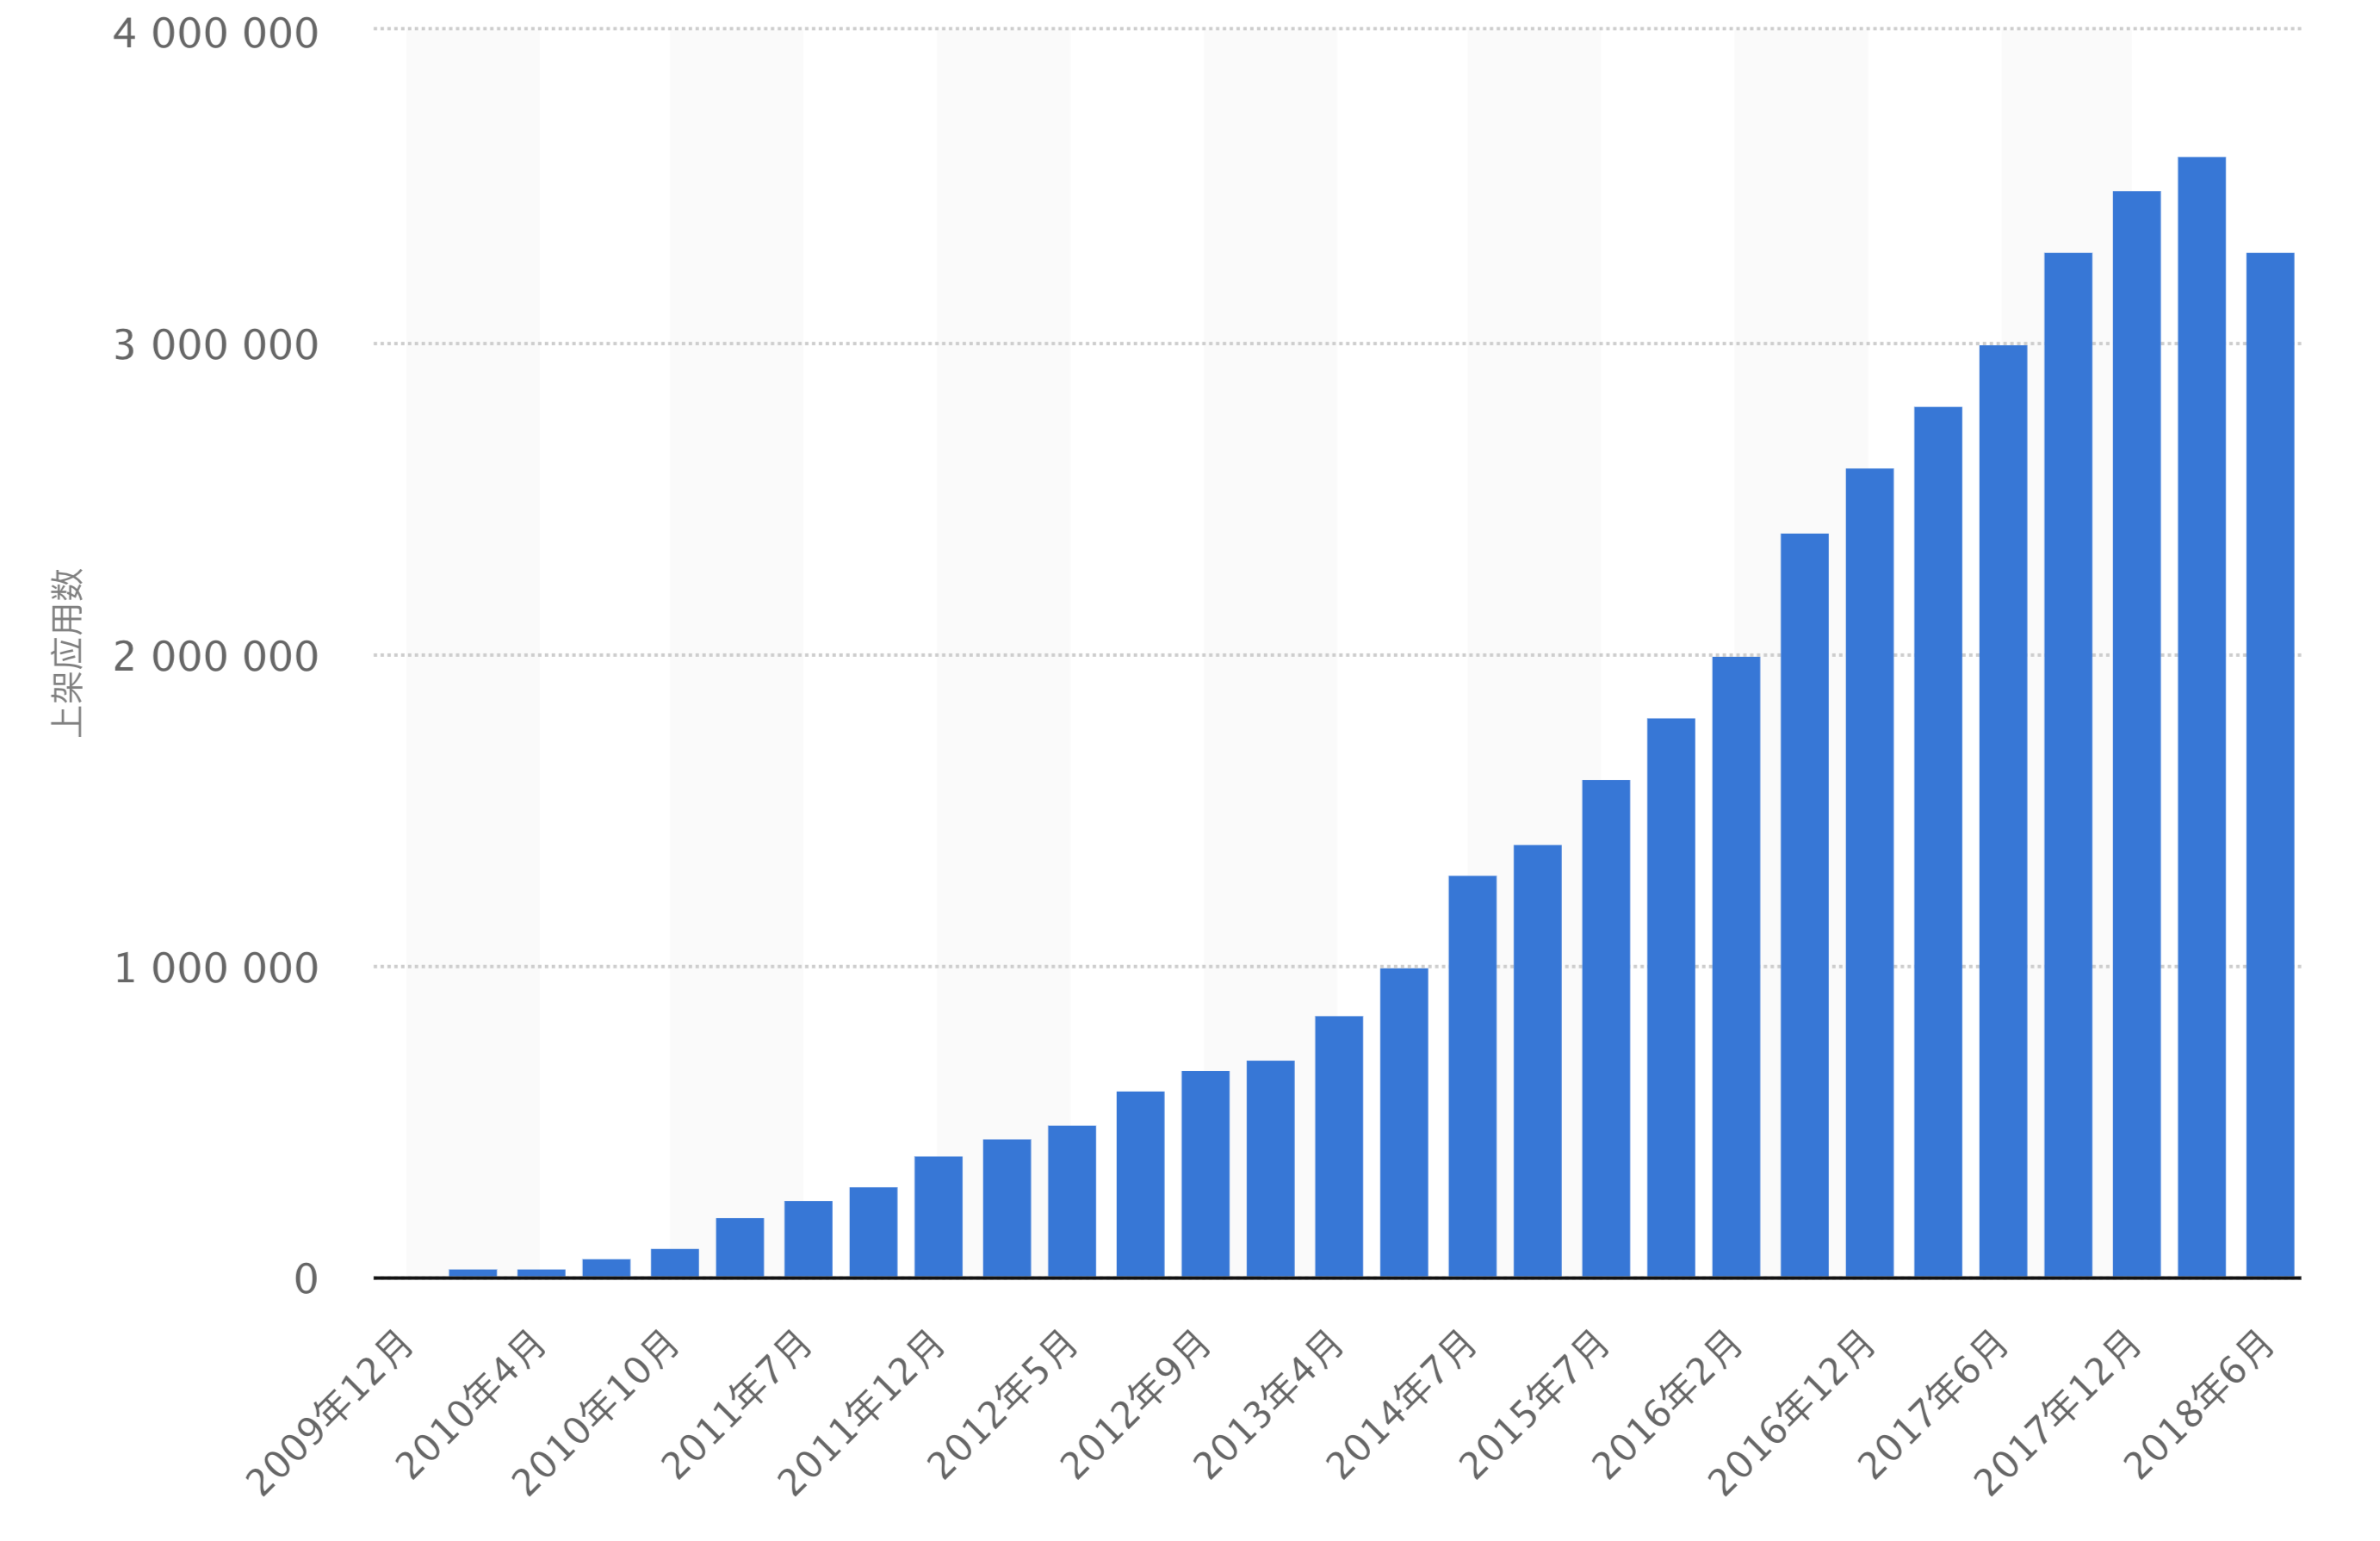
\includegraphics[width=\textwidth]{./Figures/app-numbers.png}

	\caption{Google Play Store上架的应用总数的变化趋势}
	\label{fig:app_number}
\end{figure*}


移动生活 - 移动分析方法 - 应用场景

\section{研究意义}

在Android应用的开发过程中,经常使用的面向对象编程、回调函数以及多线程交互等开发技术,会干扰Android应用静态分析工具的分析过程,导致函数调用关系的错误或者缺失。因此,仅仅依赖静态分析工具,无法准确的了解应用程序执行的具体细节。但是,传统动态分析工具对环境构建、使用成本等方面需要投入的成本大,导致开发人员难以快速上手。

为此,本文提出的解决方案,以较为便捷的方式对应用程序进行预处理,并结合具体的运行环境,从而构建Android应用程序的动态函数调用图,为研究人员提供更多样更准确的分析信息,辅助其他工具完成对Android应用程序的分析工作。这也是本文的研究意义。
\section{Android分析技术介绍}

伴随着移动互联网的兴起,国内外的研究人员开始关注移动应用分析,通过对移动应用运用软件分析技术,了解应用程序在运行过程中的行为表现。通常的,软件分析技术主要分为静态分析技术和动态分析技术两类。

\subsection{静态分析技术}
在不执行应用程序的情况下,静态分析技术通过对应用程序的源代码或者执行文件进行控制流分析和数据流分析,进而推断应用程序在运行过程中可能产生的行为。这方面相关工具包括Soot、FlowDroid、AmanDroid、IccTa等。但是,静态分析工具在分析过程中虽然可以对应用程序进行较为全面的分析,覆盖应用程序的所有代码,但由于缺少和程序执行过程相关的部分必要信息(应用程序的执行序列、和设备所处环境相关的传感器(如GPS、温度等)信息等),可能导致部分情况下分析结果的不精确。为了解决这一问题,研究人员提出了动态分析技术。

通常的,软件分析技术主要分为静态分析技术和动态分析技术两类。在不执行应用程序的情况下,静态分析技术通过对应用程序的源代码或者执行文件进行控制流分析和数据流分析,进而推断应用程序在运行过程中可能产生的行为。这方面相关工具包括Soot、FlowDroid、AmanDroid、IccTa等。Soot是传统的静态分析工具,其思路是将所有的Java字节码文件转化成一种中间语言Jimple,并在Jimple的基础上进行常规的控制流分析、数据流分析,理论上适用于所有可以在Java虚拟机上运行的语言(例如Scala、Groovy等等)的分析。由于Android程序本身的字节码Davlik和Java字节码在格式上保持一致,因此,Soot也支持Android应用程序的静态分析,但是,Soot在分析过程中没有考虑一些Android的特性难免会出现一些问题。为此,德国达姆施塔特工业大学的Steven Arzt等人在Soot的基础上考虑Android程序中Activity的生命周期特性,推出了一个针对Android的静态分析工具FlowDroid,可以做到上下文、路径、对象、字段等层面上的敏感。FlowDroid通过定义数据源点和数据泄漏点,在Android应用生命周期的基础上,可以实现数据流敏感的污点分析。但其不足之处在于缺少跨组件通信的分析不考虑多线程调用问题。在FlowDroid基础上,卢森堡大学的Li Li等人推出了IccTA,利用跨组件通信分析工具IC3提取跨组件通信(Inter-Component Communication, ICC)的方法调用,并结合AndroidManifest.xml文件定义的Intent Filter信息,连接ICC两端的组件,克服了FlowDroid因缺少跨组件通信而导致的数据流上的缺失。因为它是构建在FlowDroid之上的一个探测敏感信息泄露的,所以受限于FlowDroid的局限性。由此可见,静态分析工具在分析过程中虽然可以对应用程序进行较为全面的分析,覆盖应用程序的所有代码,但由于缺少和程序执行过程相关的部分必要信息(应用程序的执行序列、和设备所处环境相关的传感器(如GPS、温度等)信息等),可能导致部分情况下分析结果的不精确。


\subsection{动态分析技术}

为了解决这一问题,研究人员提出了动态分析技术。和静态分析技术相对应,动态分析技术通过执行应用程序,获取程序运行过程的相关信息,从而实现对应的研究目的。动态分析技术往往需要对运行环境做适当的修改或者调用特殊的系统接口,记录应用程序运行过程的关键信息,结合数据流追踪等技术,已记录应用程序的运行时行为。这一项技术通常用于恶意软件的检测和排查。这方面的工作代表包括TaintDroid 、DroidBox、TraceDroid、DroidScope等。Enck等人提出的TaintDroid通过修改Dalvik虚拟机,利用动态污点分析技术实时监控敏感数据的生成、传播和泄露,实现了变量层面、方法层面、文件层面的数据追踪。DroidBox在TaintDroid基础上,对Android Framework的部分API做了修改,可以记录一些开发人员感兴趣的API(例如文件读写、网络请求、SMS服务等)的调用,并提供分析结果的可视化。另外,DroidBox还实现了应用程序的自动安装和执行,弥补了TaintDroid在软件测试自动化方面的不足。和TaintDroid不同,TraceDroid采用的是另一种思路,利用字节码插装技术技术实现了AOP,进而根据生成的日志文件得到分析结果。

另外,还可以介绍simplepref和uber的nanoscope。

Dynamic Analysis Platforms In this section, we further explore existing dynamic analysis platforms and compare their implementations against TraceDroid. 


\begin{comment}

6.3.1 AASandbox 
In October 2010, Blasing et al. were the first to present a dynamic analysis platform for Android applications: AASandbox (Android Application Sandbox) [7]. It uses static analysis to scan software for malicious patterns and performs dynamic analysis to intervene and log low-level interactions with the system for further analysis by means of a loadable kernel module developed to obtain system call logs. AASandbox uses a system call footprinting approach for detecting suspicious applications. Unfortunately, there were no known Android malware samples available at the time to evaluate this technique. AASandbox seems to be unmaintained nowadays. Compared to AASandbox, TraceDroid is implemented on a higher abstraction layer, namely the Dalvik VM instead of the Linux kernel. This allows TraceDroid to retrieve great detail on executed Java components, while missing any native code execution paths. By using the strace utility, however, we obtain a similar overview of executed system calls. We already use analysis output to detect suspicious activity. 
6.3.2 TaintDroid 
Also in October 2010, Enck et al. presented TaintDroid: a modified Android OS keeping track of taint propagation at runtime to detect privacy leaks [26]. Over time, it has been adopted as a valuable addition by many subsequent research proposals which aim to perform dynamic analysis on Android applications. TaintDroid is implemented as a modification of the Dalvik VM and thus cannot track taint within native code. TaintDroid does not come with a set of scripts or applications to allow automated analysis and stimulation of unknown applications and is thus quite different compared to our TraceDroid platform. It does also not keep track of any specific method invocations. What we could do, however, is extending TraceDroid in such a way that it also keeps track of field operations, and use this data to implement taint tracking functionality as a post-processing plug-in. 
6.3.3 DroidBox DroidBox was developed by Patrik Lantz as part of Google Summer of Code (GSoC) 20113 . It combines TaintDroid with modifications of Android’s core libraries. The modified Android OS of DroidBox logs the following events during runtime of an application: • File read and write operations. • Cryptography API activity. • Opened network connections. • Outgoing network traffic. 3http://www.honeynet.org/node/744 78 • Information leaks through network, files or SMS messages (using TaintDroid). • Attempts to send SMS messages. • Phone calls that have been made. It also provides visualization of analysis results and automated app installation and execution. TraceDroid differs from DroidBox in that our implementation traces all method invocations, including those occurring within an application, while DroidBox looks only at a small subset of API calls of which the developers think are interesting. Our approach is beneficial, for example if malware authors use third-party cryptographic libraries instead of the hooked APIs to encrypt data. DroidBox operates on the core library level, while TraceDroid is integrated at the Dalvik bytecode interpreter. This makes TraceDroid a more suitable platform for detailed analysis of unknown applications. On top of that, our TraceDroid Analysis Platform performs a more fine-grained level of simulation techniques when compared with DroidBox. A second version of DroidBox was developed by Kun Yang as part of GSoC 2012 and introduces an APIMonitor that uses bytecode rewriting instead of core library modifications4 . While this is a good approach to overcome the need of continuously upgrading DroidBox to newer Android versions, rewriting applications breaks an app’s original signature which can easily be detected at runtime. Also, as with the first DroidBox release, the APIMonitor can only monitor core API calls which results in a less comprehensive set of traced method invocations than TraceDroid achieves. Since DroidBox was the first openly available dynamic analysis platform for Android, it has been used as a base system by many other dynamic analysis platforms including Andrubis, Mobile-Sandbox, and SandDroid. 6.3.4 Bouncer In February 2012, Google announced Bouncer [44]. It is stated that every application that is offered for download in the Google Play Store is run on Google’s cloud infrastructure and gets simulated as if it was running on an Android device. Since Bouncer is used to protect the Google Play Store from malicious applications, only sparse information was provided about its internal functioning. During Summercon in June 2012, however, Oberheide and Miller presented their efforts on dissecting Bouncer [? ]. Using a C&C application that connects back to their local machine, they determined that Bouncer runs dynamic analysis on applications for 5 minutes. They could setup a connect-back shell to communicate with the application under investigation5 and were able to obtain more detailed information on the environment used by Bouncer to run analysis. In October 2012, Google introduced an application verification service. With the release of Android 4.2, the ACTION PACKAGE NEEDS VERIFICATION broadcast was introduced, used by the OS to verify newly installed applications and check them for known malware. During installation, th the app (including its package name and its SHA1 hash) and the device (its ID and IP address) to the Google cloud and requests a verification response. Although not confirmed, the Google cloud likely uses Bouncer results to make statements about the app’s safety. A study performed by Xuxian Jiang shows that only 193 of the 1260 malgenome samples were detected as malicious by this verification scheme, indicating a detection rate of only 15.32%6 6.3.5 Andrubis In June 2012, the International Secure Systems Lab released Andrubis: a dynamic analysis platform for Android applications [42]. Andrubis was the first to offer a publicly available web interface where users can submit Android applications for dynamic analysis. When analysis is finished, it generates a XML report containing a behavioral and static analysis footprint of the requested application. Its first release was based on DroidBox’s core library modifications and was built on top of Android 2.1. Andrubis was later updated to run under Android 2.3.4 and uses VMI to intercept system calls made by native code execution. With the integration of TraceDroid, Andrubis has become a very extensive dynamic analysis platform that does not only track taint propagation to detect privacy leaks, but also records invoked system calls and comprehensive Java method traces. Due to our collaboration efforts, Andrubis has adopted most of TraceDroid’s functionality. 6.3.6 DroidScope First presented in August 2012, DroidScope is a comprehensive dynamic binary instrumentation tool for Android based on VM introspection [72]. It reconstructs Dalvik instruction traces and this could, in theory, be used to obtain the same results as we currently obtain with TraceDroid. The key difference between TraceDroid and DroidScope, however, is the fact that DroidScope is bound to an emulator, while TraceDroid may run on actual hardware. Malicious applications can detect the use of an emulator and may decide not to start malicious activities in this scenario [55]. 6.3.7 AppsPlayground In February 2013, Rastogi et al. introduce AppsPlayground. Like previously discussed frameworks, AppsPlayground monitors taint propagation using TaintDroid, and traces specific Java API and system calls. Its main contribution is an improved monkey exerciser-like execution approach to explore application’s GUIs. The latter is something we would like to add to our TraceDroid Analysis Platform as well, as a mean to increase code coverage. 6.3.8 Mobile-Sandbox Mobile-Sandbox was released in March 2013 and is very similar to Andrubis in that it is based on DroidBox and uses TaintDroid to track taint propagation [64]. Instead of VMI to trace system calls, however, Mobile-Sandbox 6http://www.cs.ncsu.edu/faculty/jiang/appverify 80 uses a ported version of ltrace to trace native library invocations. This ltrace binary may be a valuable addition to our TraceDroid analysis platform. Like Andrubis, Mobile-Sandbox also allows users to submit Android applications for analysis via a web application. 6.3.9 CopperDroid Finally, in April 2013, Reina et al. introduced CopperDroid [58]. The mechanisms used in this system are similar to DroidScope as it also uses VMI to collect system call information about analyzed applications. Reina et al. argue, however, that CopperDroid points out how their system call-centric analysis and stimulation techniques can comprehensively expose Android malware behaviors. CopperDroid also comes with a web interface where users can submit unknown applications for analysis. 6.3.10 Closed frameworks A number of additional dynamic analysis platforms have been implemented and made available to the public via web applications. These frameworks, however, come with very little documentation on how they operate which makes it hard to make statements on any new approaches used by these implementations. It is likely that these platforms use (modified versions of) existing tools like DroidBox, TaintDroid and Androguard to complement their dynamic analysis engine. This is confirmed on SandDroid’s webpage, which states that it is powered by both DroidBox and Androguard7 . Example output reports of both ForeSafe8 and JoeSecurity9 suggest that these platforms use a combination of existing tools as well.

\end{comment}

\section{基于上述分析技术的应用}

\textbf{应用分类:}

\textbf{安全性分析:}

- 漏洞检查

- 

\textbf{质量保障:}

% 例如错误定位、自动化分析、profiling等

\section{本文的主要工作}

本文的主要研究工作包括以下:

1)	调研最近几年Android应用分析领域的静动态分析工具,了解各项工具的优劣以及相关的应用案例。

2)	提出并实现Android动态函数调用图构建系统,包含传统函数调用图的构建以及在此基础之上的多线程函数调用关系的构建。

3)	对上述系统设计对应的实验方案,评估对应的实验效果。

\section{本文的组织结构}

本文共分为六章,环绕着Android动态函数调用图构建系统的设计与实现展开,各章节内容如下:

第一章主要介绍了本文的主要研究背景、主要工作内容以及研究意义,最后对本文的各章的内容做了阐述。

第二章从Android的体系结构出发,并由此展开介绍了最近几年Android领域相关的静态分析技术和动态分析技术,以及这些技术在各自领域的运用,简单描述本文可能遇到的困难。

第三章从系统功能、技术路线、技术选型、模块实现等若干方面介绍RunDroid的设计与实现。

第四章从应用程序的构建效率、日志本身记录效率以及系统对程序运行的影响等三个方面设计并开展相关的测试实验。

第五章将展示RunDroid系统生成的函数调用图的运行结果,并对函数调用图进行详细的阐述。

第六章对本文工作进行总结,并对下一步工作进行展望。

\cleardoublepage
\chapter{Android系统相关背景介绍 }  
\label{ch2}


本章首先会简要介绍Android系统架构,其次会对Android中的Activity组件做基本介绍,接着会着重介绍Android中常见的两种多线程交互方式,最后将指出本文系统在实现上的难点。

\section{Android系统结构介绍}

Android是基于Linux内核开发的的开源操作系统,隶属于Google公司,主要用于触屏移动设备如智能手机、平板电脑与其他便携式设备,是目前世界上最流行的移动终端操作系统之一。

在系统架构上,Android自下到上,可以分为四层:Kernel层、Library和Android Runtime(Dalvik/ART)、Framework、Application等,如~\autoref{fig:Android-Framework}所示。
Kernel层是硬件和软件层之间的抽象层,主要是设备的驱动程序,例如:显示驱动、音频驱动、蓝牙驱动、Binder IPC驱动等。
Library和Android Runtime(Dalvik/ART): Library,顾名思义就是向上层提供各种这样的基础功能,例如SQLite数据库引擎,Surface Manager显示系统管理库。
Android Runtime主要是运行Android程序的虚拟机,在不同版本的系统上对应着不同的虚拟机,例如在Android 5.0及以上是ART,而在Android 4.3及以下是Dalvik,而Android 4.4两者都有。
Framework层主要是系统管理类库,包括Activity的管理,消息通知的管理;同时,它是Application的基础架构,为应用程序层的开发者提供了API,其存在简化了程序的开发。
而Application就是我们平时接触的应用,开发人员公国调用底层Framework提供的API实现相应的接口。

虽然Android应用程序是使用Java语言开发的,但是它和传统的Java程序有着很大的不同,具体有如下几点:

\begin{figure*}
	\centering
	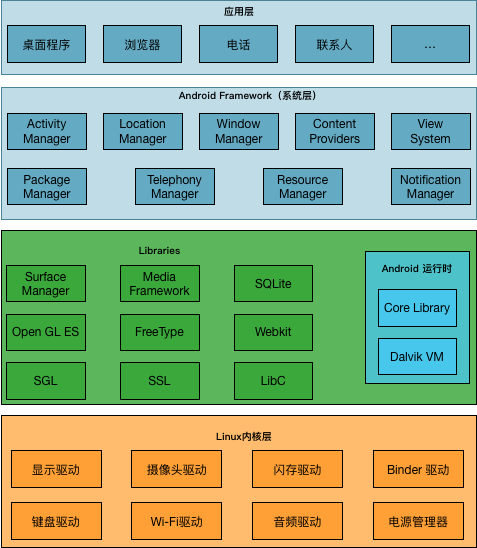
\includegraphics[width=\textwidth]{./Figures/Android-Framework.png}
	\caption{Android系统框架图}
	\label{fig:Android-Framework}
\end{figure*}


\textbf{异于常规程序的开发方式:}
在设计上,Android应用程序的开发架构采用的是事件驱动架构。在开发过程中,没有传统程序中入口函数Entry Point的概念。应用程序中通用的业务逻辑(例如应用程序如何启动退出、应用的窗口如何创建销毁等)存在于Android Framework中。这也使得Android应用程序的分发文件(即APK文件)相对较小。

\textbf{面向组件的开发方式:}
Android程序中较为常见的是组件(Component,例如Activity、Service、Content Provider、Broadcast Receiver),它是应用程序运行的最小单元,受到Android Framework的直接调度。开发人员通过继承这些组件,重写对应的生命周期函数,已实现对应的业务需求(界面的布局、页面状态的保存等),而这些组件的生命周期由Framework调度完成。

\textbf{大量逻辑实现依赖于回调函数和多线程通信:}
由于Android应用程序采用的是基于单线程消息队列的事件驱动架构,因此,界面相关的操作只允许出现在主线程(UI Thread)中,耗时操作只能在工作线程(Worker Thread)中进行。通常的,开发人员往往会借助回调函数处理控件的响应事件,利用多线程交互串联界面相关操作和耗时操作,完成对应的业务。


\section{Android中的Activity}

在Android应用程序运行过程中,Activity向用户展示图形界面,响应用户的反馈,和其他组件一同完成相关业务,扮演着最为重要的作用。由于Android应用程序在架构选型上采用了事件驱动模型,为了便于协调应用内部状态的管理,Android组件通常有生命周期的概念,Activity也不例外。

Android系统根据Activity 在运行时和用户的反馈将其状态分为以下四种:
\begin{enumerate}

\item 运行态:在该状态下, Activity处于页面最前端时,用户可以与Activity进行交互。一般的,我们看到Activity均处于这个状态。

\item 暂停态:在该状态,Activity仍然可见,但是失去了窗口的焦点。当一个Activity之上出现一个透明的Activity、Toast或者对话框时,Activity就处于这个状态。处于暂停状态的Activity仍处于存活状态,保存着所有的内存数据,只有当系统内存极度紧张时,才有可能被系统杀死回收。

\item 停止态:当一个Activity被其他的Activity遮挡时,处于这个状态。处于该状态的Activity仍然可以保留所有的状态,只是对用户不可见。系统在需要内存的情况下,可以采用相应的策略对Activity进行杀死回收操作。

\item 终止态:当Activity处于暂停态或者停止态时,系统由于内存原因可能会将上述两种Activity杀死回收。处于该状态下的Activity将不能直接恢复。
\end{enumerate}

Activity的生命周期就是以上状态之间的跳转,受到Activity在运行时的内存分布、环境状态以及业务逻辑的影响,由Android系统直接负责调度。
Android系统为Activity提供了onCreate(), onStart(), onResume(), onPaused(), onRestart(),  onStoped()和onDestroy()等方法,方便开发人员在Activity的状态发生变化时对程序的运行时数据和应用状态做适当的处理操作。对应的Activity的生命周期具体如~\autoref{fig:Activity-lifecycle}所示:

 
\begin{figure*}
	\centering
	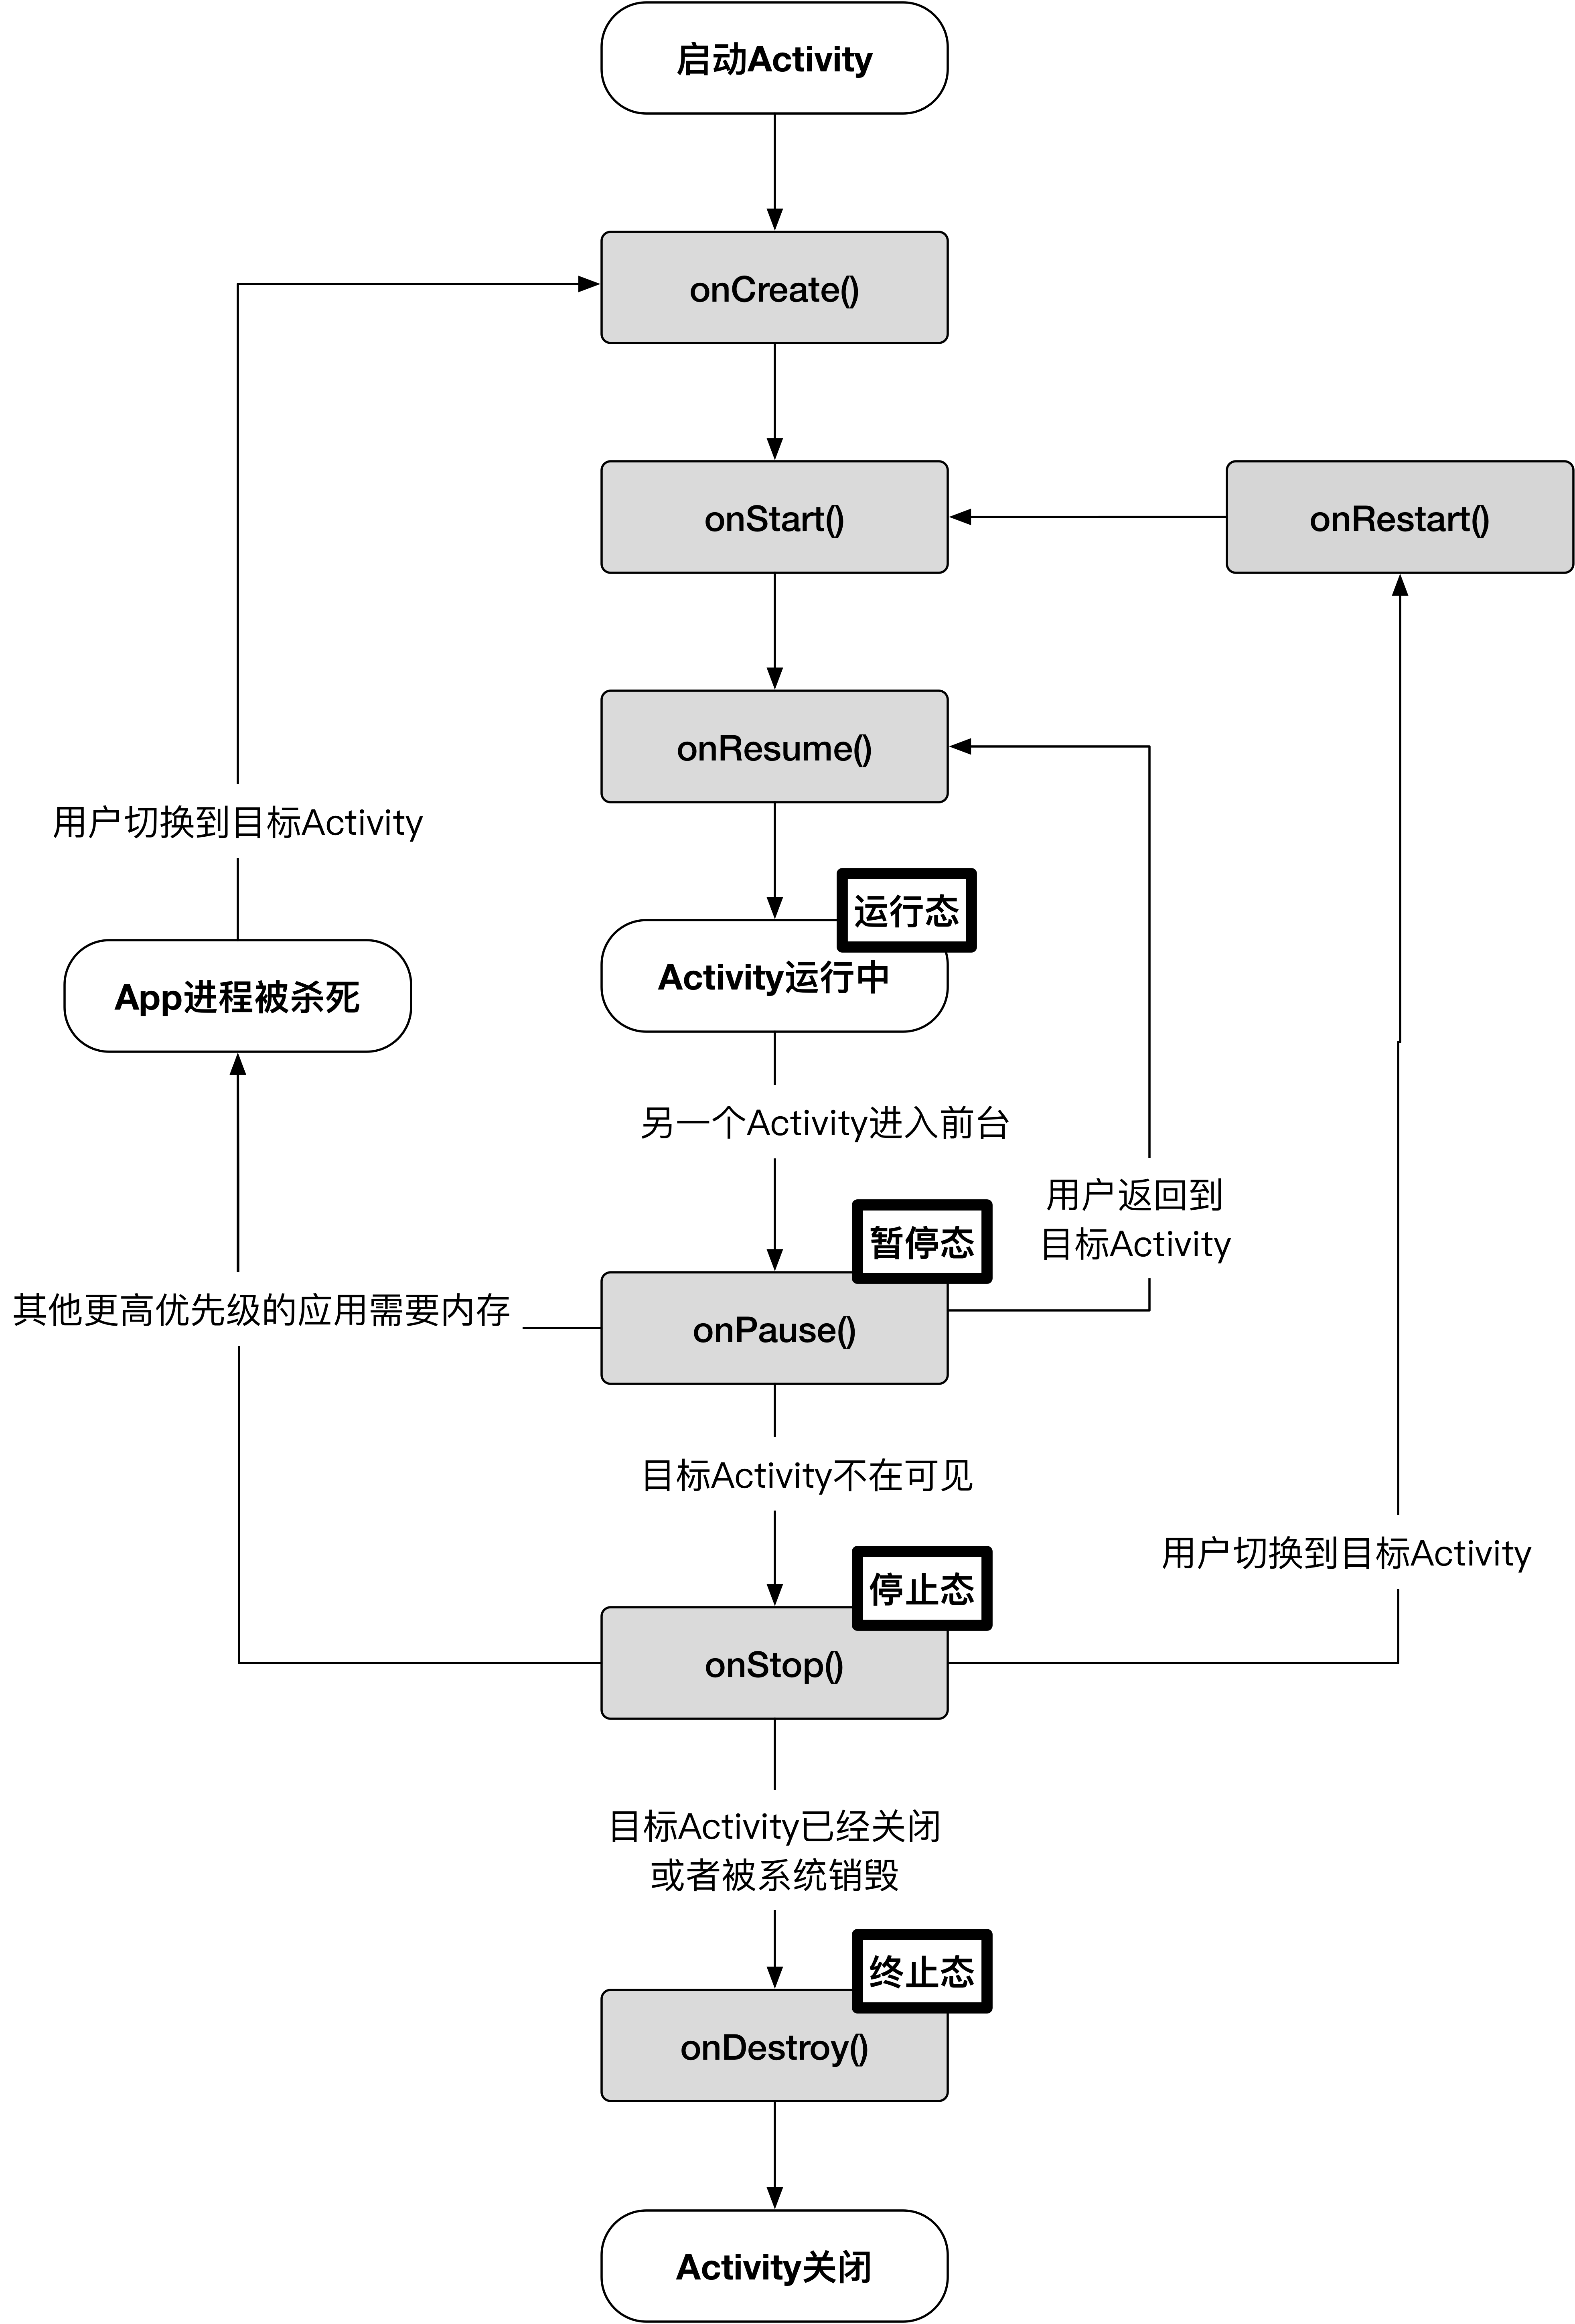
\includegraphics[width=\textwidth]{./Figures/Activity-lifecycle.png}
	\caption{Activity的生命周期}
	\label{fig:Activity-lifecycle}
\end{figure*}


当用户点击应用图标,系统启动应用程序后,系统会创建Activity、启动Activity并使之可以和用户进行交互,在这个过程中,onCreate()、onStart()、onResume()等方法被回调,Activity最终处于运行态;

当用户点击“返回键”返回到桌面时,Activity会失去焦点,在用户的视野中消失,直至被系统回收,对应的状态也从运行态经暂停态、停止态,变为终止态变,期间onPause()、onStop()、onDestroy等方法被回调;

当用户从一个界面回到原来的界面时,原有的Activity从停止态重启,先后出现在设备界面上,获得和用户交互的焦点,期间onRestart()、onStart()、onResume()等方法被回调;

当一个Activity长期处于停止态,但由于内存原因被系统回收时,用户尝试启动它时,系统会像启动一个新的Activity一样启动它。

\section{Android中的多线程交互}
 Android系统在架构设计上采用了事件驱动架构。在多线程并发访问时,若UI控件对于各线程均是可见的,并发对控件做读写操作会使控件处于不可预期的状态;若贸然对控件使用锁机制,这将会使阻塞部分线程业务逻辑的执行,使得应用变得复杂低效。上述情况对于应用程序都是不可接受的。为了避免多线程操作之间的竞争关系带来的低效率问题,Android系统在设计事件驱动架构时,采用了单线程的消息队列,即只允许在主线程(也称为主线程,Main Thread)进行界面更新操作,不允许在其他线程(也称为工作线程,Worker Thread)进行界面更新操作。

当应用程序出现耗时操作(例如加载磁盘上的图片、网络请求等)时,应用程序往往需要在一个新的线程中执行上述逻辑。当应用程序界面中的某些控件需要根据耗时操作的结果(例如渲染得到的图片对象、网络请求得到的JSON字段)更新界面状态时,开发人员需要切换到主线程进行界面的更新。

从整体上,开发者可以需要的交互方式分为基于Java的多线程交互和基于Handler的交互方式。

\subsection{基于Java的多线程交互}

由于Android系统提供的API接口兼容Java多线程相关的部分API,因此,在Android系统中,开发人员可以采用和Java应用相同的调用方式启动工作线程,并在对应的线程上完成业务逻辑。但是,Java API只能实现业务逻辑从原有线程转移到新的工作线程上,不能重新返回到主线程上。为此,Android系统在Java API的基础上还提供了void runOnUiThread (Runnable action) API。runOnUiThread API可以帮助开发人员将业务逻辑的执行从工作线程转移到主线程上,该API也符合Android只允许在主线程上更新界面这一基本设计原则。但是,该API也存在着一些弊端,例如runOnUiThread API的定义位于类android.app.Activity,这也就意味着在Android组件Service中进行耗时操作时,无法通过该API返回到主线程;同时基于接口的函数参数定义方式对于跨线程的参数传递也不是十分友好。为此,Android提供了基于Handler的多线程交互方式。

\subsection{基于Handler的多线程消息调度}

为了满足开发人员多样化的业务在多线程间的切换,Android提供了基于Handler消息调度的多线程交互方式。当开发人员需要当前业务逻辑转移到其他线程时,通过方法Message.obtain()获取一个Message,将对应的业务逻辑封装成Runnable对象传递给Message中对应的字段,或者将对应的参数传递给Message中的参数字段,最后通过Handler对象发送给指定的消息队列。当目标线程的消息队列读取到这条消息时,便会在该线程中执行预定的业务逻辑。

~\autoref{fig:handler-code}为Handler的简单示例:用户在工作线程执行一项耗时任务(生成一个字符串),将生成的字符串传递给Message对象,并通过Handler对象通知主线程进行界面更新。
 
 
\begin{figure*}[h]
	\centering
	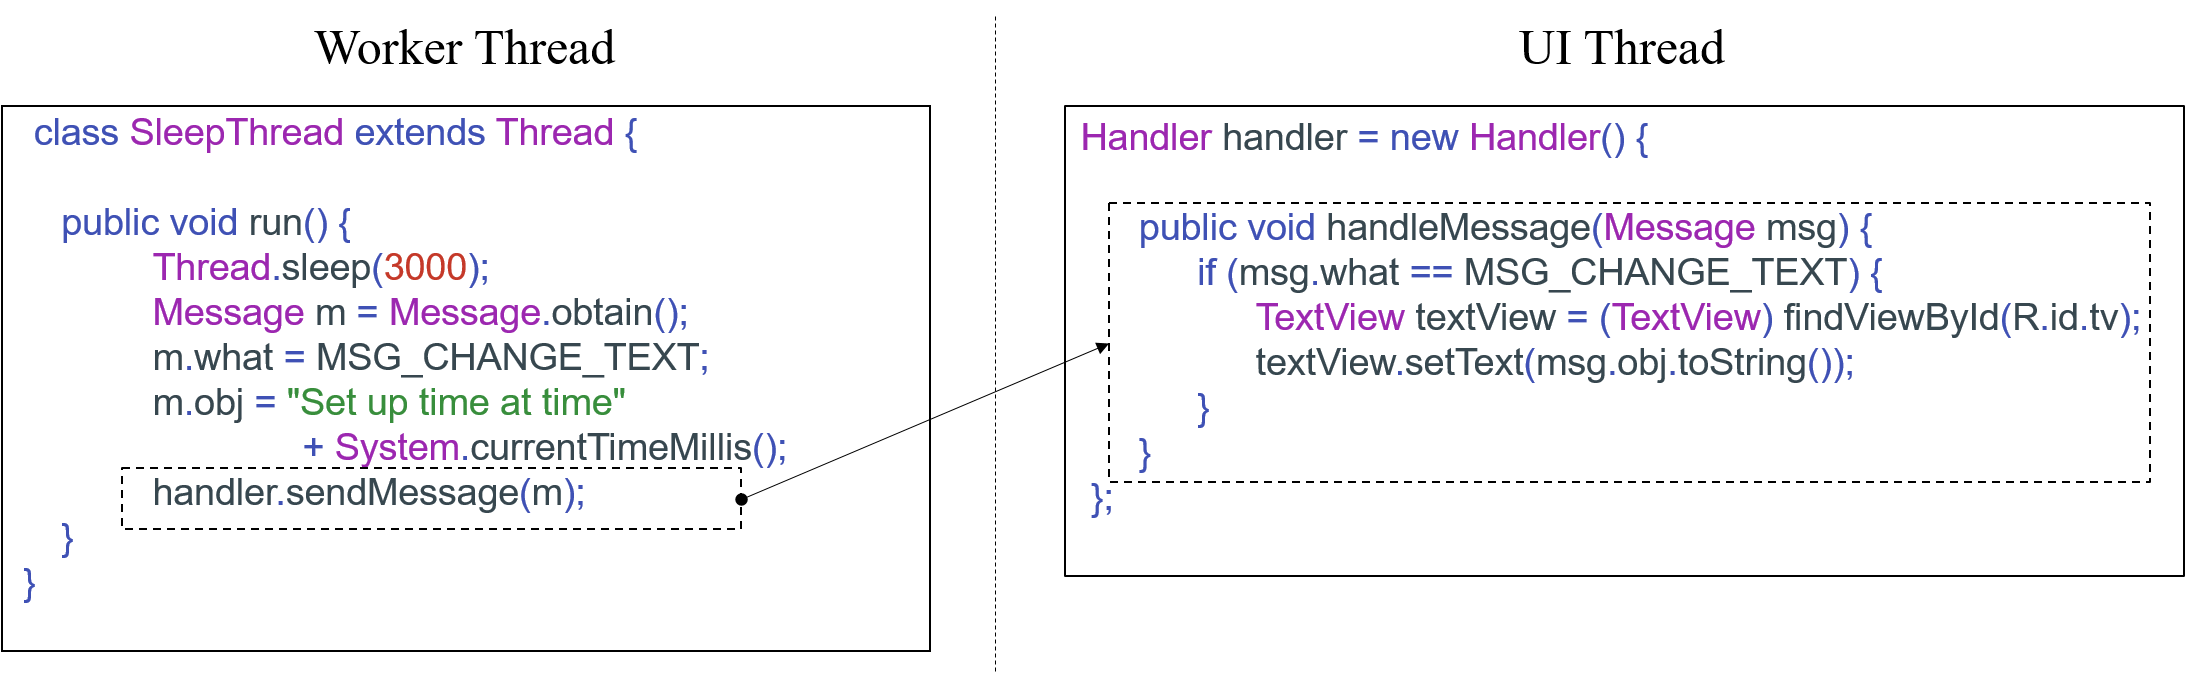
\includegraphics[width=\textwidth]{./Figures/handler-code.png}
	\caption{Handler的使用实例}
	\label{fig:handler-code}
\end{figure*}


从Android SDK提供的API来看,开发人员可以通过post(Runnable),postAtTime(Runnable,long),sendMessage(Message),postDelayed(Runnable, Object, long), sendMessageDelayed(Message,long),sendMessageAtTime(Message,long)和sendEmptyMessage(int)等多种API形式实现消息调度。通过查阅和分析Android系统相关源代码,我们发现上述Handler相关的API关系如~\autoref{fig:handler-apis}所示。

 
 \begin{figure*}[h]
	\centering
	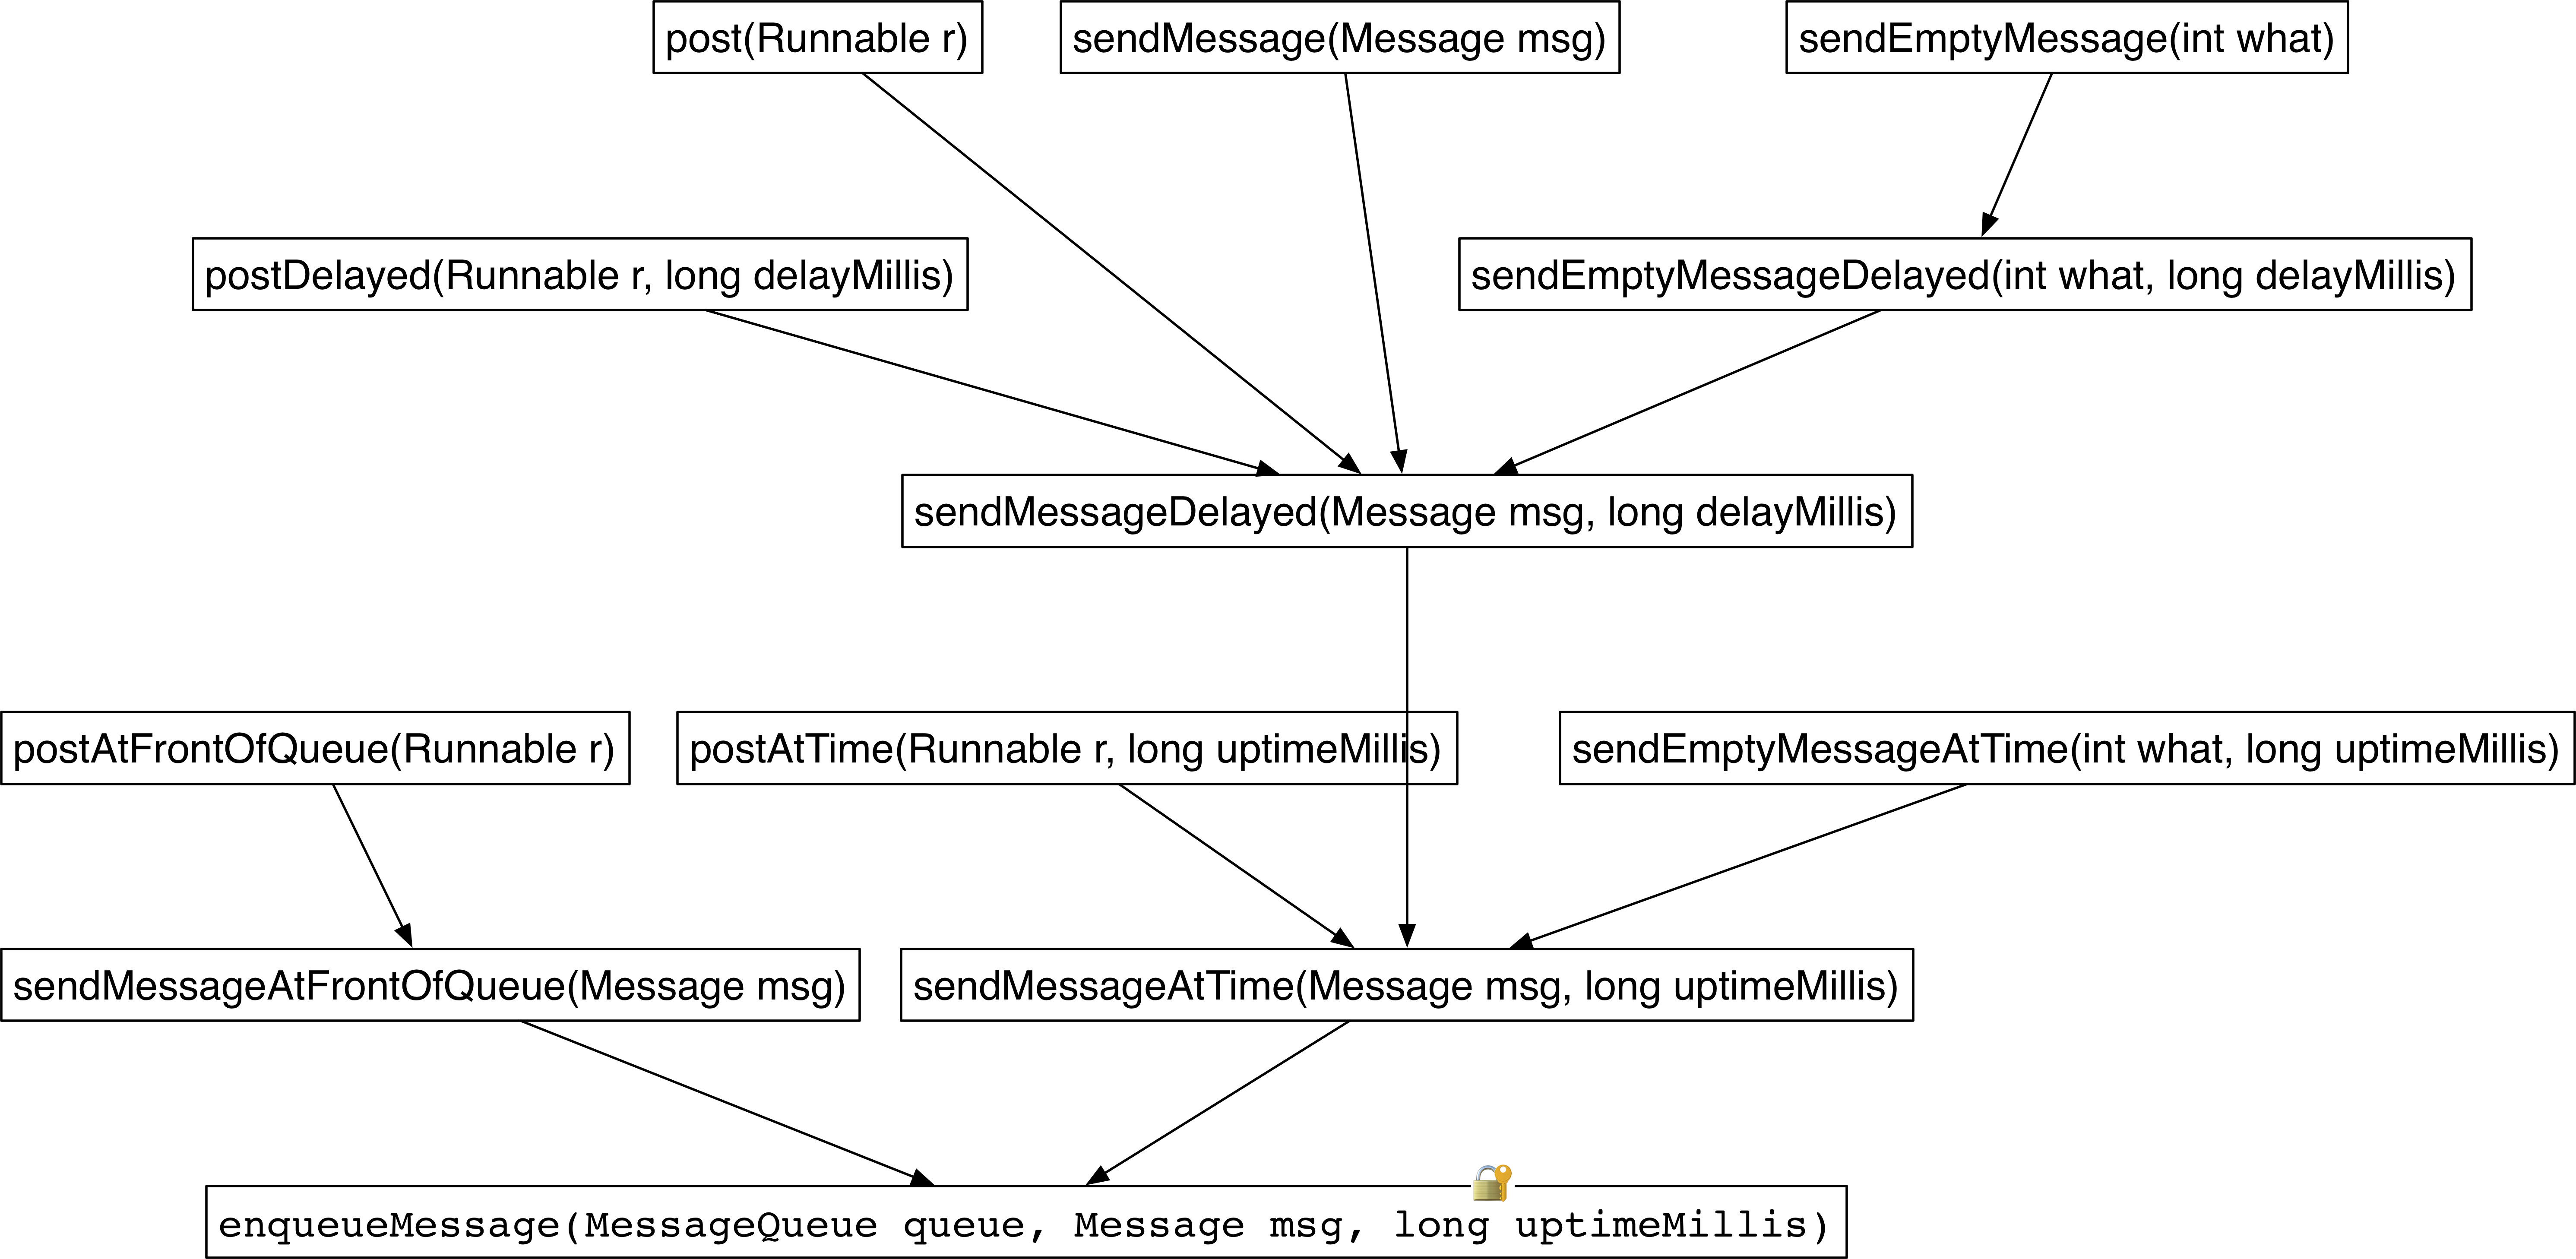
\includegraphics[width=\textwidth]{./Figures/Handler-apis.png}
	\caption{ Handler 各API之间的调用关系}
	\label{fig:handler-apis}
\end{figure*}


从~\autoref{fig:handler-apis}中,我们可以发现所有的API最后就会调用到android.os.Handler enqueueMessage(MessageQueue, Message, long)方法。

从底层实现上看,Handler机制主要由Handler、Looper、MessageQueue、Message等若干部分组成。Message是跨线程交互的主要载体,Android系统采用对象池的设计模式来管理Message对象;无论开发人员以何种形式调用了Handler发送消息,传递的参数最后均会封装到Message对象中。MessageQueue则存放着所有待处理的Message对象,它是一个双端队列,开发人员可以根据具体业务场景在消息队列的头部、尾部或者适当位置插入消息队列。Looper则负责以epoll的方式从MessageQueue中循环读取Message对象,分发给对应的Handler对象使得业务可以在对应恰当的线程上被处理;一个线程最多只允许只有一个Looper对象,他只能绑定一个与之对应的MessageQueue;其中最为常见的就是位于主线程的MainLooper,它主要负责Android系统的日常调度(例如Activity的生命周期、控件的点击事件响应等)。Handler对象则负责将消息发送到对应的MessageQueue中(扮演着消息的生产者角色)以及消费来自Looper分发下来的Message(扮演着消息的消费者角色);在一个应用中,Handler可以存在多个对象,一个Handler对象也可以同时扮演生产者和消费者两个角色。

从原理上看,基于Handler的多线程消息调度,充分利用了Android的事件驱动架构,将业务逻辑抽象出Message对象。该消息对象通过Handler的对应接口发送至在目标线程所对应的消息队列MessageQueue中,再由Looper对象在目标线程运行时从消息队列中取出,分发给对应的Handler执行,达到了Android跨线程交互的目的。具体地,Handler的工作原理如~\autoref{fig:handler-framework}所示:
 

 \begin{figure*}[h]
	\centering
	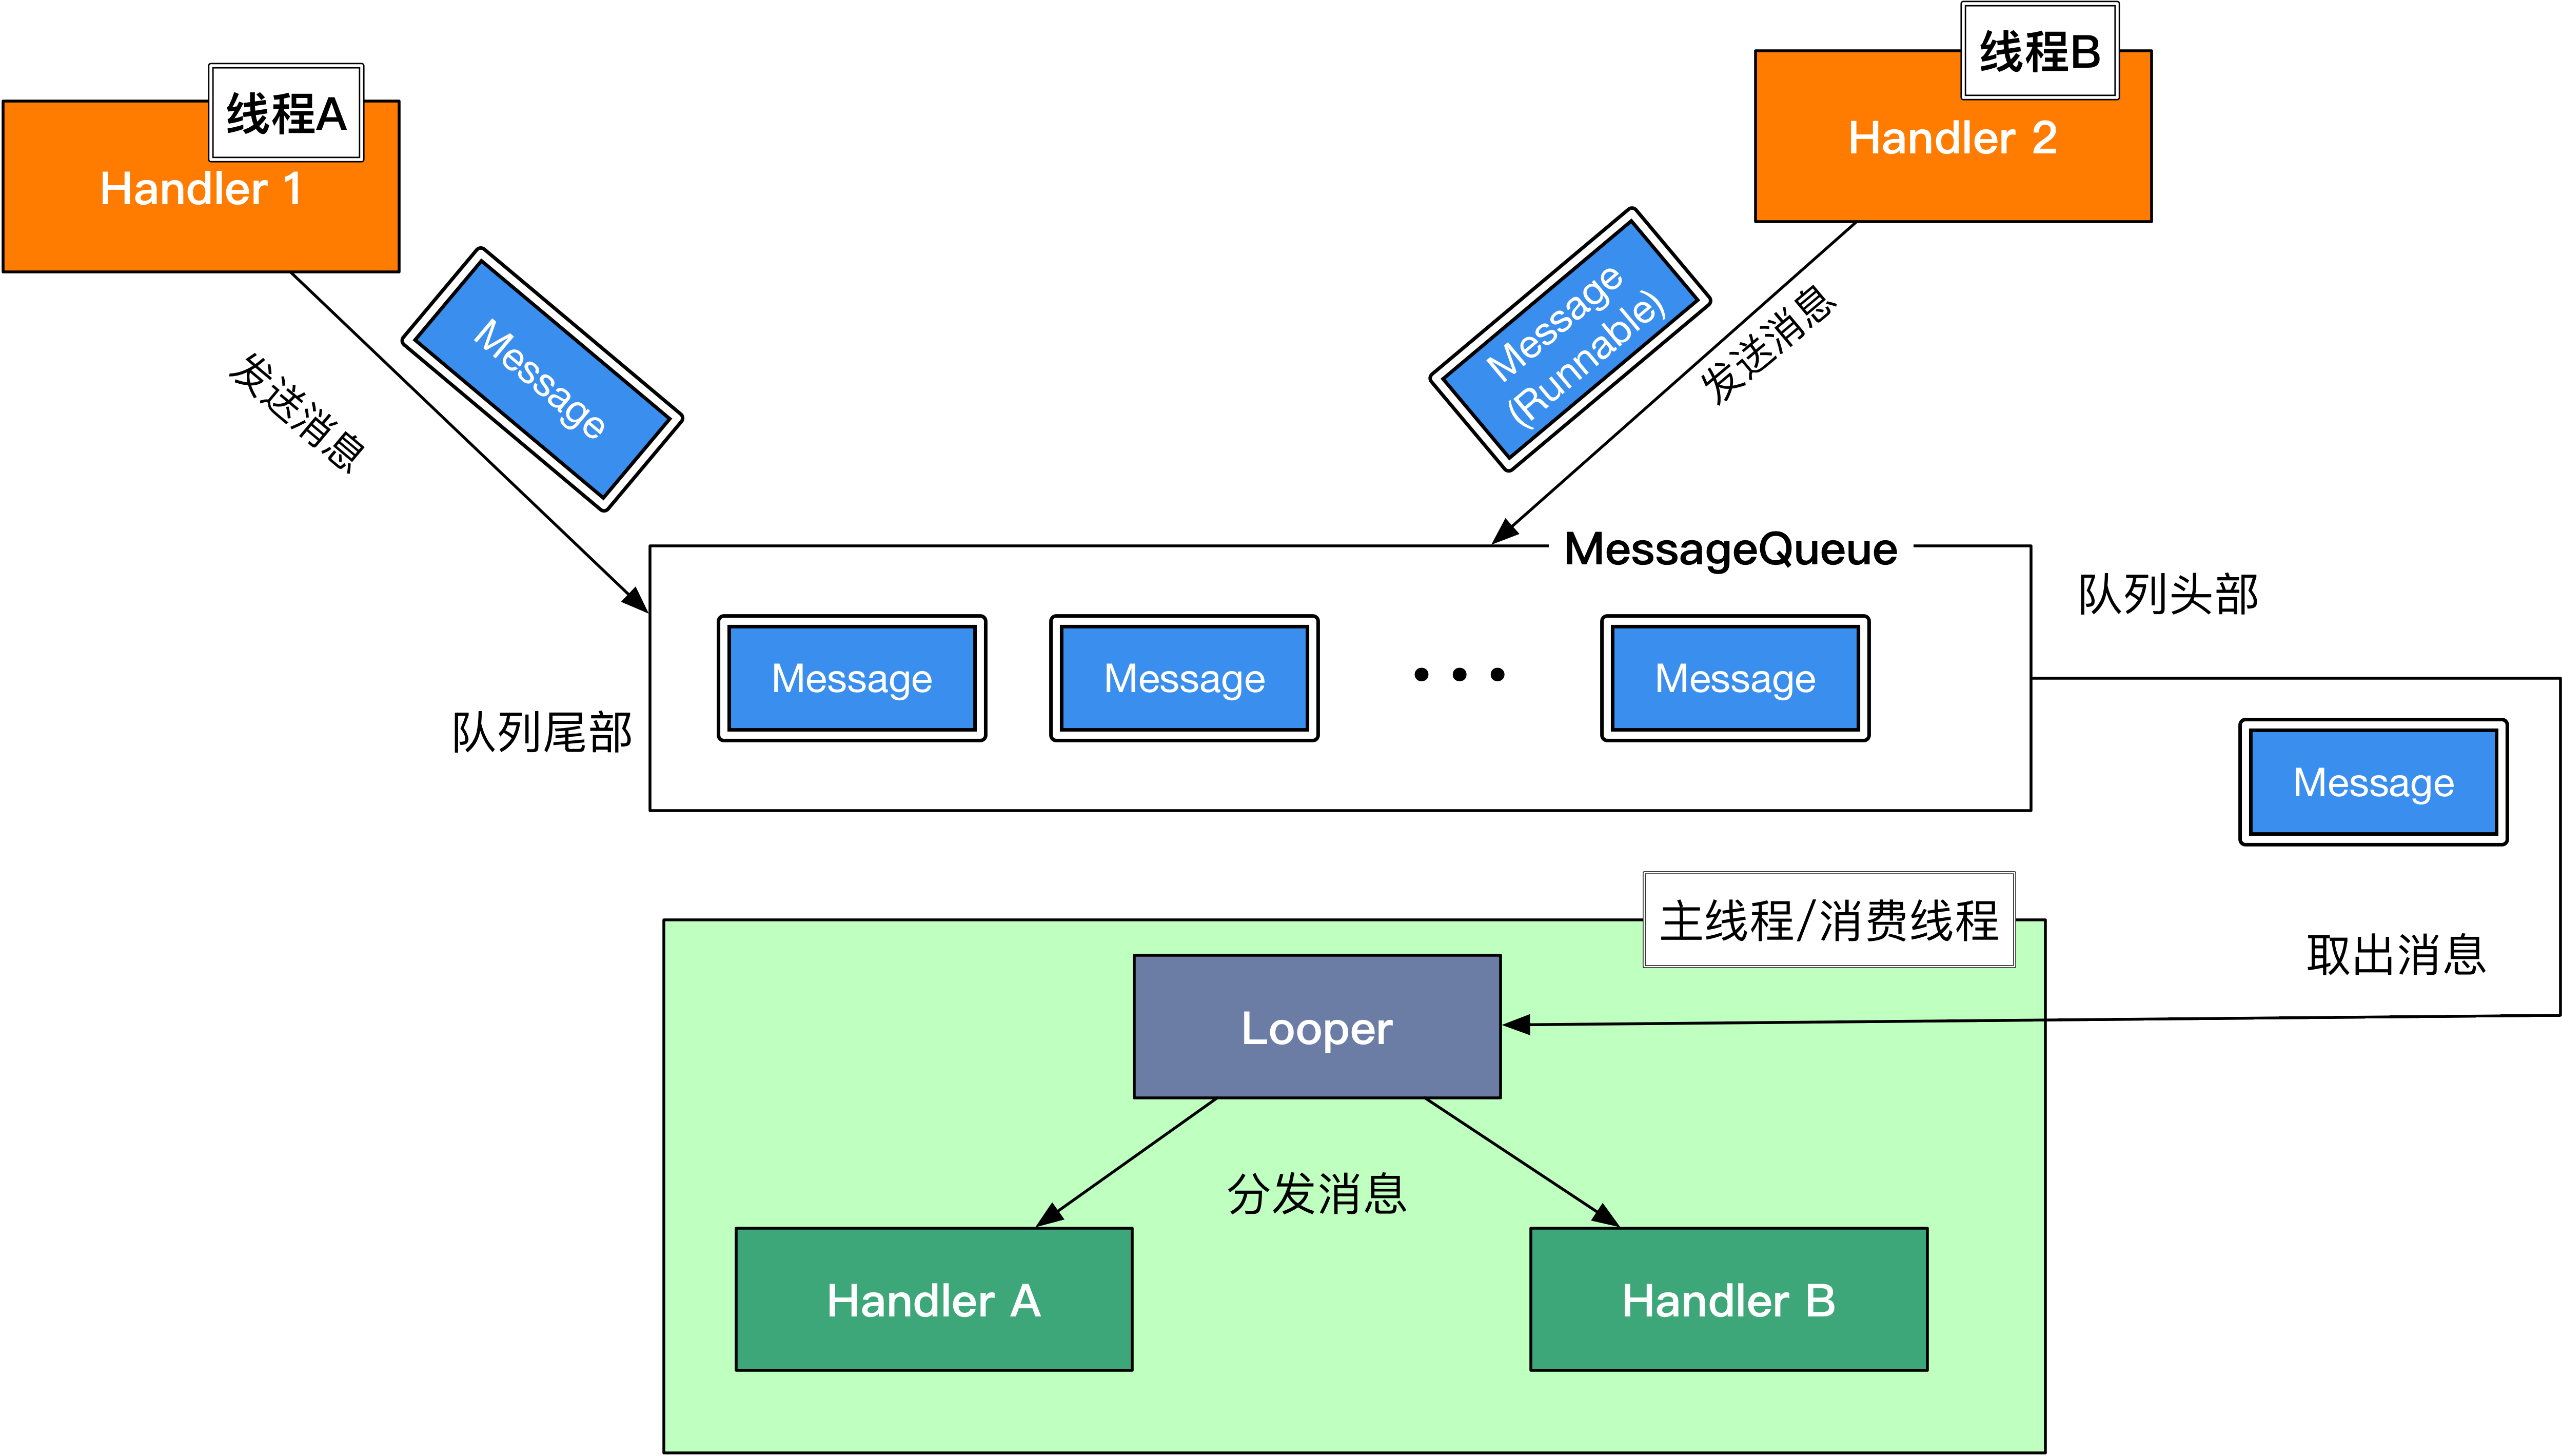
\includegraphics[width=\textwidth]{./Figures/Handler-framework.png}
	\caption{ Handler的工作原理}
	\label{fig:handler-framework}
\end{figure*}


综上所述,基于Handler消息调度的多线程交互方式,不仅可以帮助开发人员实现业务逻辑在主线程和工作线程间的自由转移,而且其灵活的API设计还帮助开发人员降低应用的设计复杂程度,提升了系统架构的可拓展性。因此,在Android开发过程中,基于Handler消息调度的多线程交互十分常见。
\section{本文遇到的困难与挑战}


 本文解决的关键问题有如下几点:

1)	如何获取应用程序中各个函数的执行信息?

获取应用程序在执行过程中各函数执行信息是本文的基础。从函数分类上,用户定义的方法和系统预定义的方法。对于前者,我们可以通过修改程序源代码实现;但对于后者,由于我们无法直接修改系统程序的源代码或者构建一个符合本文业务需求的系统的成本较高,为此,我们需要寻找对应的解决方案以帮助我们获取系统方法的执行信息。

2)	如何根据程序中各函数的的执行信息,还原应用程序的函数调用图?

基于第一点,我们可以获取程序在运行过程中的执行信息。但仅仅依靠这些执行信息是不够的,我们还需要将这些执行信息组织起来,挖掘执行信息之间的关联关系,从而才能还原成应用程序的函数调用图。这将是本文研究的重点之一。

3)	如何在生成的函数调用图中体现Android特性?

正如上文所提的,Android系统中有很多常规应用中不具备的特性,例如Activity的生命周期、基于多线程调用的触发关系。若要在生成的函数调用图上体现上述特性,需要对Android系统源代码有一定的了解熟悉,并基于图中的相关信息创建与特性相对应的关系,这既是本文研究的重点,也是本文的创新点。

\section{本章小结}

本章主要介绍了Android系统的相关背景知识,较为详细的阐述了Android的系统结构,详细介绍了Android四大组件之一的Activity机器生命周期。同时,本章还介绍了基于Runnable/Thread、Handler消息调度两种不同的多线程交互方式,较为详细地分析了Handler的运行机制,为下文基于函数调用图的多线程触发关系生成做了铺垫。最后,本章还介绍了系统在实现上可能遇到的困难。

\cleardoublepage
\section{RunDroid系统的设计与实现 }
\label{ch3}

\subsection{系统功能介绍}
本文以帮助研究人员和开发人员了解Android应用程序的执行过程作为基本出发点,通过设计与实现Android动态函数调用图构建系统RunDroid,生成Android应用程序运行时对应的动态函数调用图,从方法调用关系、方法间的触发关系以及方法执行的相关对象信息等多个方面较为全面地展现Android应用的执行过程,为应用程序分析提供更为多样、准确的信息。另外,系统具备一定的可拓展性,可以方便相关人员根据自身的业务需求对系统进行扩展,完成相应的需求。

\subsection{概念定义}
\eat{
\define{
    图:图是是对节点和边的描述,通常使用二元组$G(V,E)$表示。对于图中的节点$v$, $v \in V$;对于图中的边 $e$, $e \in E$。
}
\define{
    有向图:按照图中的边是否区分方向,我们可以将图分为有向图和无向图。
}
}


\define{
    调用(Invoke):对于程序$P$的两个方法$m_1$和$m_2$,如果在方法$m_1$中调用了方法$m_2$,则记作$m_1 \to m_2$,称为方法$m_1$调用方法$m_2$。
}
\begin{equation}
m_0 \to m_1 \to \dots m_{n - 1} \to m_n  \label{equ:extend_invoke}
\end{equation}

    在此基础上,对于方法$m_0$和方法$m_n$,若存在方法$m_i$($i=1,\dots,n-1,n>1$),使得~\ref{equ:extend_invoke}成立,,则记作$m_0 \stackrel{\ast}{\to} m_n$,称为方法$m_0$扩展调用方法$m_n$。


    补充的,对于方法$m_1$和方法$m_2$,若$m_1 \to m_2$,也可以记为$m_1  \stackrel{\ast}{\to}  m_2$。

\define{
    函数调用图(CallGraph,CG):函数调用图$CG = ( V , E)$是一个有向图(DAG), 图中的点$ v \in V $表示一个\textbf{方法实体} $m$;
    如果方法$m_1$调用方法$m_2$(即$m_1 \to m_2$),则有向边 $e = (m_1 ,m_2)$属于集合 $E$。 
}

\define{
    动态函数调用图(Dynamic CallGraph,DCG):动态函数调用图是在调用图的基础上演化而来,是对程序运行时行为的描述。
    同样的,动态函数调用图也是一个有向图($DCG = ( V , E)$)。 图中的点$ v \in V $表示一个\textbf{方法执行} $m$;
    如果方法$m_1$调用方法$m_2$(即$m_1 \to m_2$),则有向边 $e = (m_1 ,m_2)$属于集合 $E$。 
}

\textbf{注意:}函数调用图和动态函数调用图是分别从静态分析角度和动态分析角度对程序运行过程的描述。
前者分析的整体是方法实体,是静态分析的结果,每次产生的结果是一样的;
后台则为方法执行,是对动态行为的描述,每次产生的结果和具体的执行过程相关,不一定是一样的。

例如,方法A调用了方法B,函数调用图$CG$如~\ref{equ:cg_sample}所示。
但若,在实际执行过程中,方法A被调用了两次,这对应的动态函数调用图$DCG$如~\ref{equ:dcg_sample}所示。
可以看出,$DCG$中,$method_a$ 和 $method_b$ 各有两个,分别对应的两次\textbf{函数执行}。
\begin{equation}
CG = ({method_a,method_b},{(method_a \to method_b )} ) \label{equ:cg_sample}
\end{equation}

\begin{equation}
\begin{aligned}
DCG = &(V,G) ,\\ 
V = & \{method_{a_{(1)}},method_{b_{(1)}},method_{a_{(2)}},method_{b_{(2)}}\}, \\ 
G = & \{  
    (  method_{a_{(1)}} \to method_{b_{(1)}}) ,( method_{a_{(2)}} \to method_{b_{(2)}})
 \} 
\end{aligned}
\label{equ:dcg_sample} 
\end{equation}


\define{
    方法对象(Method Object,MO):
和方法执行相关的对象称为方法对象,可以体现对象和执行方法的相互关系。
具体的,在一次具体的方法执行过程中,
如果对象$p$是这个方法$m$的参数,记为$p \stackrel{parameter}{\longrightarrow} m$;
如果对象$r$是这个方法$m$的返回值,记为$r \stackrel{return}{\longrightarrow} m$;
若方法$m$是非静态方法,则方法执行时我们可以获取到关联到的this指针对象$i$,记为$i \stackrel{instance}{\longrightarrow} m$;
}


\define{
    触发关系(Trigger):
    如果对于动态函数调用图$DCG$中两个方法(不妨记为$m_a$和$m_b$,$m_a \in DCG$,$m_b \in DCG $),若方法$m_a$和方法$m_b$之间同时需要满足以下三个条件,
    则两个方法存在触发关系,记为$m_a \hookrightarrow m_b$,称为$m_a$触发了$m_b$:
    
\begin{enumerate}
  \item 方法$m_a$的执行时间总是在方法$m_b$的执行时间之前;
  \item $m_a \stackrel{\ast}{\to} m_b $不成立;
  \item $m_a$、$m_b$之间存在着一定的因果关系,包括但不限于生命周期事件,UI交互事件或多线程通信等。
\end{enumerate}
}

\define{
    拓展动态函数调用图(Extended Dynamic CallGraph,EDCG):在动态函数调用图(DCG)的基础上,添加了方法对象和函数间的触发关系。
    拓展动态函数调用图中的节点包括方法执行节点和方法对象节点。图中的边包括描述方法间关系的边和描述方法和对象间的边:
    前者的方法间关系包括调用关系和触发关系;而后者的关系包括和方法对象相关的三个关系。
    具体定义如~\ref{equ:def_edcg}所示:

\begin{equation}
\begin{aligned}
EDCG = & (V_{EDCG},E_{EDCG}) ,\\ 
DCG = & (V_{DCG},E_{DCG}) ,\\ 
V_{EDCG} = & V_{method} \bigcup V_{object} ,\\
V_{method} = & V_{DCG}, \\ 
G_{EDCG} = & G_{method} \bigcup G_{object} , \\
G_{method} = & E_{DCG} \bigcup \{ (m_1 , m_2) m_1 \hookrightarrow m_2 \}
\end{aligned}
\label{equ:def_edcg} 
\end{equation}
    
}

\subsection{ 设计思路介绍}
以下面一段代码里为例,我们将简要介绍一下RunDroid还原Android应用程序动态函数调用图的基本思路:
~\ref{fig:code_sample}-左为一段面向过程编程的示例代码,当main函数执行时,会一次调用A、B两个函数,而B函数有调用了C、D两个函数,
对应动态函数调用图如~\ref{fig:code_sample}-右所示。
 
 
 \begin{figure*}
	\centering
	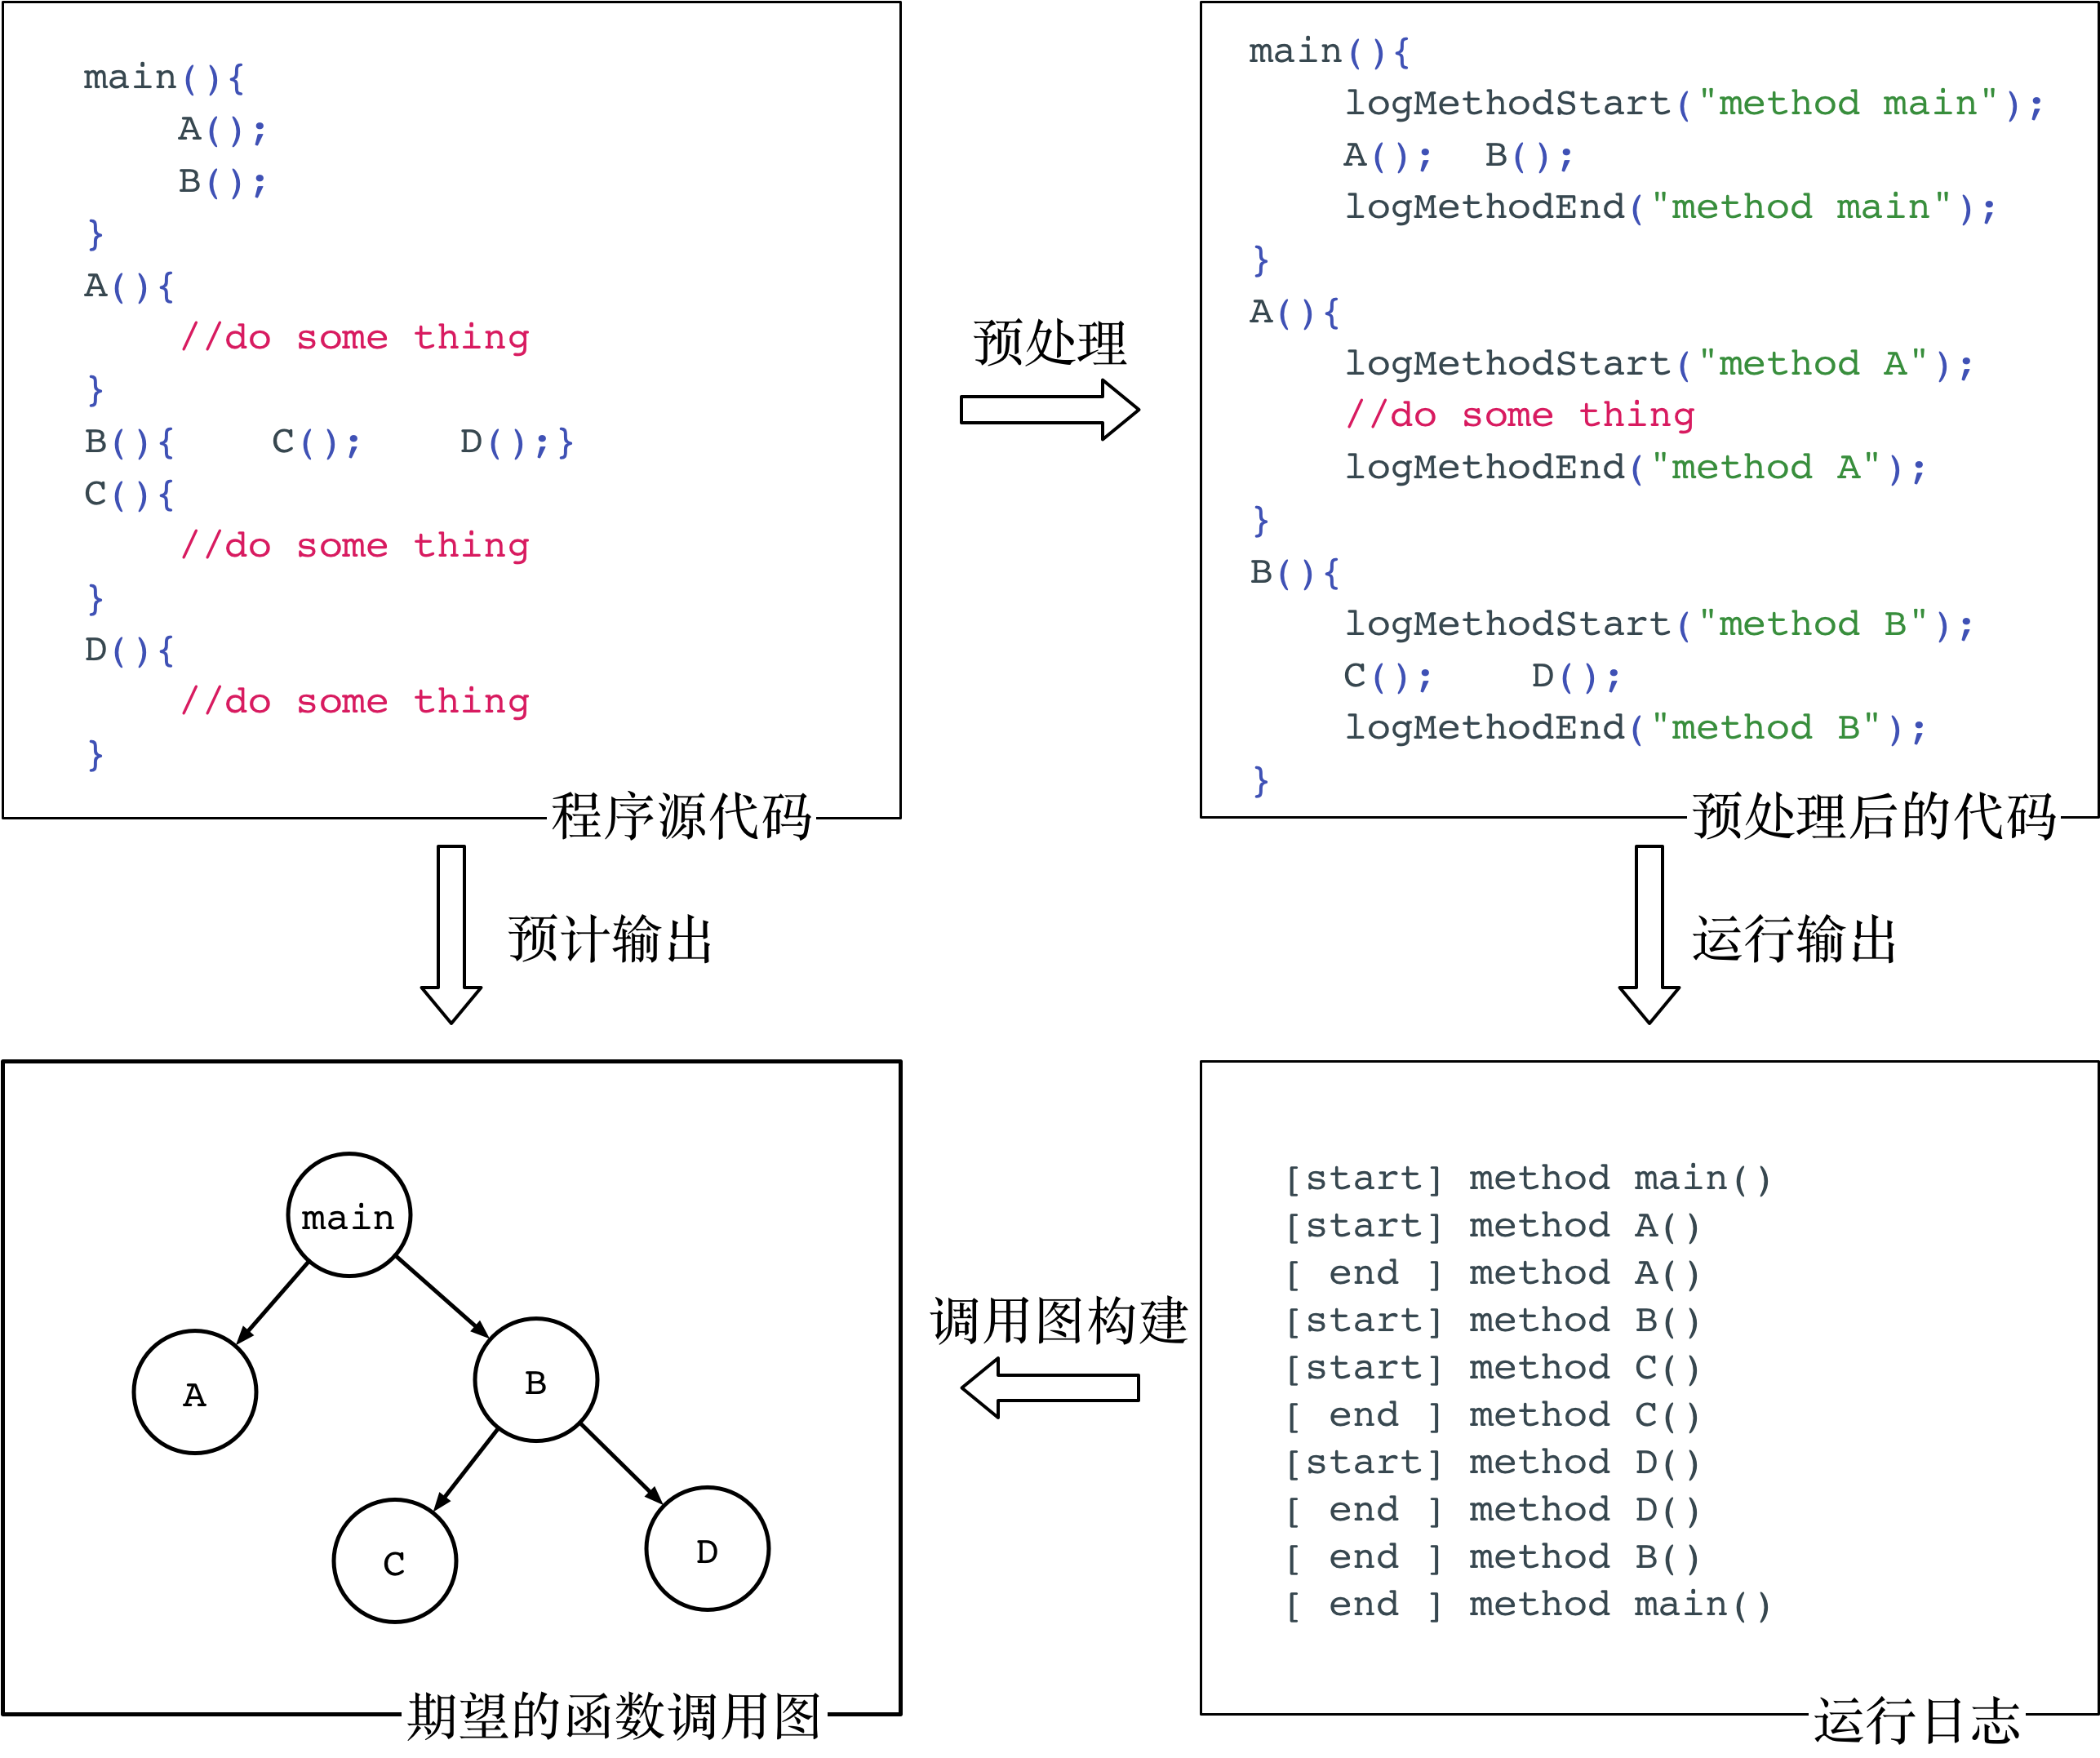
\includegraphics[width=\textwidth]{./Figures/code-sample.png}
	\caption{ 面向过程编程语言的函数调用的示例}
	\label{fig:code_sample}
\end{figure*}


从函数调用图的构建过程可以看出,程序的执行过程就是对函数调用图自上而下的深度优先遍历过程。由此可见,若要还原出图 6-右中的函数调用图,本文采用的基本思路是以日志方式输出对右图中的函数调用图的深度优先遍历序列,并基于得到的遍历序列还原出函数调用图。
由于Android是由面向对象编程语言Java开发的系统,系统还需要考虑面向对象编程的特性——多态性(即同一个行为在不同的对象下的表现可以不同)。为此,RunDroid还会在函数调用图将函数执行和对应的对象进行关联,更好地体现面向对象编程的函数调用关系。基于上述的函数调用关系的信息,RunDroid根据函数调用之间的关系进一步挖掘,进一步挖掘Android系统中的特性(例如组件Activity的生命周期、多线程的交互方式)。

\subsection{技术路线(偏工程性)}
本技术路线拟利用语法分析工具,对Android应用程序进行了应用源代码层面的执行日志插桩工作,利用非侵入式系统行为修改插件获取系统层面的函数执行信息。结合以上日志信息,方案对日志进行初步处理,在图数据库上构建原始的Android应用程序的动态函数调用图。通过阅读分析Android系统中多线程相关的源代码,制定具体的多线程分析插件,进而在函数调用图中标识出多线程相关的方法间触发关系,全面地展现Android应用的执行过程。
 
 
\begin{figure*}
\centering
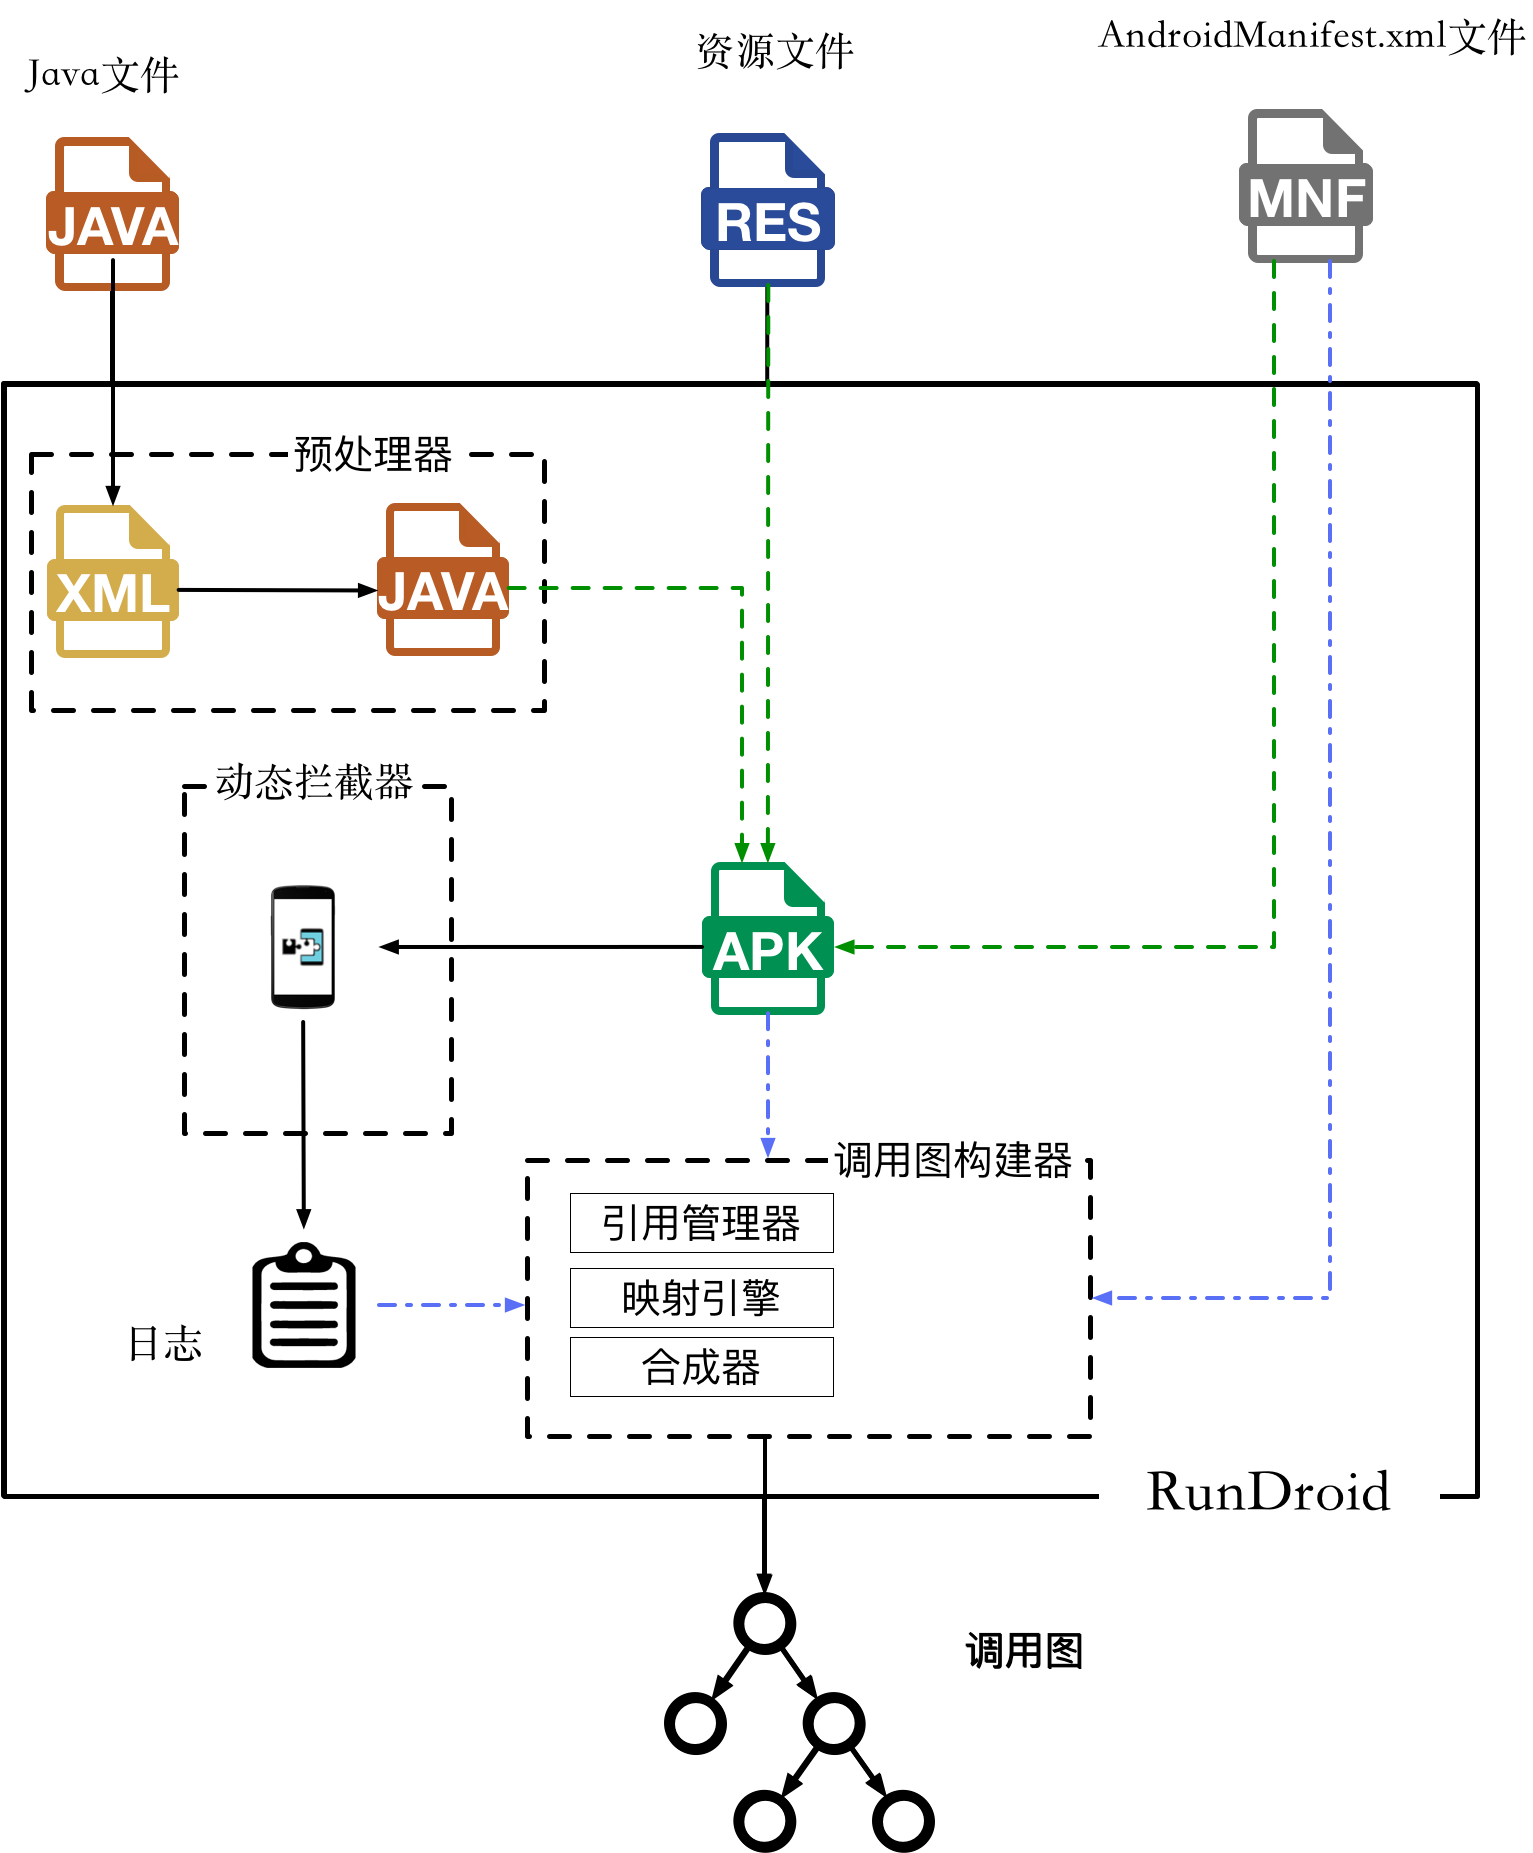
\includegraphics[width=\textwidth]{./Figures/rundroid-overview.png}
\caption{ RunDroid基本架构图}
\label{fig:rundroid_overview}
\end{figure*}


\subsection{相关技术介绍}

\subsubsection{	srcML介绍}

\subsubsection{Xposed框架介绍}
Xposed是由rovo89主导开发的第三方框架。基于Xposed开发的第三方插件,可以在不修改系统和应用程序源代码的情况下,改变他们的运行行为。Xposed框架可以运行在不同版本的Android系统上,开发过程十分便利,而且易于撤销。Xposed的实现原理具体如下:由于Android系统的所有的应用程序进程都是由Zygote进程孵化而来,Xposed通过替换/system/bin/app\_process程序,使得系统在启动过程中加载Xposed的相关文件,将所有的目标方法指向Native方法xposedCallHandler,维护目标方法和对应的钩子方法(Hook Function)的映射关系,从而实现对Zygote进程及Dalvik虚拟机的劫持;当程序执行到目标方法时,xposedCallHandler会完成目标方法的原有代码和对应钩子方法的调度,达到对目标方法劫持的目的。使用Xposed,可以帮助我们实现类似面向切面编程(Aspect-Oriented Programming, AOP)的功能,完成系统层面的方法执行情况的记录。
\subsubsection{	Neo4j介绍}
Neo4j是基于Java语言开发的图数据库。与传统的基于关系模型的存储结构不同,Neo4j的存储模型是基于图论开发的,遵循属性图数据模型。Neo4j的数据主要分为节点(Node)和关系(Relationship)两大类,另外,Neo4j还可以在关系和节点上添加key-value形式的属性,为节点指定一个或者多个标签,为关系指定类型等等。Neo4j以Lucence作为索引支撑,支持完整的 ACID(原子性,一致性,隔离性和持久性)事务规则,提供了基于Cypher脚本、Native Java API和REST Http API等多种方式帮助开发人员进行数据开发工作。同时,Neo4j还提供了友好的浏览器界面,具有十分友好的交互体验。由于基于属性图数据模型,Neo4j通常适用于和图关系有着密切关系的应用场景:例如社交网络分析,公共交通网络研究以及地图网络拓扑等场景。在RunDroid,Neo4j主要承担着函数调用图的数据存储和查询的主要职责。

\subsection{模块实现介绍}


\subsubsection{源代码预处理组件(Preprocessor)}

\subsubsection{	运行时日志记录器(Runtime Logger)}

\subsubsection{调用图构建器(Call-graph Builder)}

\subsection{构建过程介绍}


\subsubsection{如何构建函数调用图}

算法:
输入:
输出:
过程:
写一段
写一段
写一段
写一段
写一段
写一段
写一段

\subsubsection{如何构建Activity的生命周期}

\subsubsection{	如何构建多线程触发关系}

\subsection{本章小结}

\cleardoublepage
\chapter{X}  
\label{ch4}


\cleardoublepage
\section{X}
\label{ch5}

\cleardoublepage
\chapter{总结与展望}  
\label{ch6}


\section{总结}

本文尝试提出一个Android动态函数调用图构建系统,从应用层和系统层对Android应用程序的执行过程进行记录,并利用得到的执行日志信息还原Android应用程序的动态函数调用图,从方法层面还原程序的执行过程。
另外,通过Android系统的源代码进行分析,我们可以找到Android应用程序中多线程相关的函数触发关系,进一步全面的展现Android应用程序的执行过程。
另外,开发人员还可以对系统进行拓展,实现自身的需求。

\section{展望}

\cleardoublepage
\section{X }
\label{ch7}





\cleardoublepage

 \rhead[]{\heiti{华东师范大学硕士学位论文}}
 \lhead[\heiti{华东师范大学硕士学位论文}]{}
\phantomsection

\addcontentsline{toc}{chapter}{参考文献}
\bibliography{sigproc}


\cleardoublepage

\phantomsection
%\rhead[致谢]{ The performance of new graduates}
% \lhead[致谢]{ The performance of new graduates}

\addcontentsline{toc}{chapter}{致谢}
{\kaishu
{\chapter*{\vspace{-3cm} 致\qquad 谢}}

\vspace{-0.5cm}

\begin{center} 
\end{center}
	
	在此论文完成之际,我首先要感谢我的导师杜德慧。她严肃的科学态度,严谨的治学精神以及精益求精的工作作风深深地感染和激励着我。从课题的选择到项目的最终完成,杜老师都始终给予我细心的指导和不懈的支持。两年来,她不仅在学业上给我以精心指导,同时还在思想、生活上给我以无微不至的关怀与照顾,在此谨向杜老师致以诚挚的谢意和崇高的敬意。

	感谢在研究生学习期间给我诸多教诲和帮助的软件学院的各位老师和同学、以及和我一起生活两年的室友,你们的执着、勤奋、以及对生活的态度,值得我学习。特别的,我要感谢辅导员张炜帆对我思想以及生活上的帮助,给我带来了莫大的帮助。

	最后感谢我的家人,你们不仅给我经济上的支持,同时还在我成长道路上无私地给予莫大支持与鼓励,让我独立地选择自己的人生道路。

\vspace{0.2cm} \hspace{11.5cm} 

\hspace{10.6cm}  二〇一七年十月 }



\cleardoublepage
\phantomsection
\addcontentsline{toc}{chapter}{攻读硕士学位期间发表论文和参与科研情况}
\section*{攻读硕士学位期间发表论文}

\vskip 5mm

{\heiti $\blacksquare$ 已公开发表论文}\vskip 5mm

\begin{enumerate}

  \item Yujie Yuan, Lihua Xu, Xusheng Xiao, Andy Podgurski, and Huibiao Zhu,RunDroid: Recovering Execution Call Graphs for Android Applications. In Proc. ESEC/FSE, 2017
  \eat{
  	\item xxxx  Proceedings of the IEEE Conference on Computer Vision and Pattern Recognition xxxxx 为模式识别和计算机视觉的三大国际顶级会议,中国计算机协会列为A类会议,根据猲猰猱猷年谷歌学术统计,h5-index排名所有学术刊物第35位,位列工程和计算机领域所有学术刊物第一位。 
  	注:第二作者,导师第一作者。xxxx是中国计算机协 会A类、图像处理领域的顶级期刊,SCI II区。
  }

\end{enumerate}




%\printindex



\end{document}
